\chapter{Diseño}\label{ch:diseño}
%************************************************
En este capitulo se pretende abordar la principal tarea del diseño o la planificación de la estructura idónea sobre las necesidades que se han ido explicando en capítulos anteriores. Para ello se intentará plantear las decisiones tomadas desde un nivel alto, eligiendo la estructura o arquitectura correcta, bajando gradualmente hasta encajar todos los componentes, con el objetivo de obrar un sistema escalable y ágil que proporcione la solución a los problemas supuestos del cliente.

\section{Arquitectura planteada}
La necesidades que se han ido explicando en capítulos anteriores se pueden dividir en diferentes aplicaciones, funcionalidades o divisiones de capas. Cada aplicación debe funcionar cumpliendo un único objetivo, pero finalmente deben coaccionar como una sola aplicación para el usuario final. Las distintas funcionalidades que surgen ante las necesidades que se explicaron anteriormente se pueden dividir en tres tipos (operaciones de datos, su gestión y su visualización). Al tratar de construir una aplicación que requiere muchas capas horizontales independientes y a la vez que puedan interactuar entre ellas, el patrón de software que surge ante esta necesidad es el patrón arquitectónico en capas. Además de ser un patrón muy común en el ámbito web, es bastante sencillo de entender e implementar. Cada capa tiene un papel determinado y una responsabilidad específica dentro de la aplicación, dichas capas pueden cooperar e interactuar entre si, pero no dependen una de otra. Se debe saber que una capa de nivel superior puede interactuar con la capa de nivel inferior, pero no al revés. \cite{aqruitecturaMicrosoft}

\vspace{0.3cm}

Por norma general, las capas de una aplicación tienen la posibilidad de residir en una sola maquina física (misma capa) o pueden estar compartidas sobre diferentes máquinas (n-capas). En nuestro caso, la solución más óptima sería n-capas, debido a la posibilidad de mejorar la escalabilidad y optimización. Además, al dividir el proyecto por capas se mejora la flexibilidad y se puede usar en diferentes plataformas como servicio, esto último debido a que es fácilmente portable. Gracias a ello se puede dar uso de \ac{PaaS} como Vercel, Heroku o MongoDB Atlas, consiguiendo numerosas ventajas ya que se facilita la configuración, el despliegue, las tareas de automatización y el escalado.

\vspace{0.3cm}

La arquitectura de n-capas se suele dividir en tres. Las necesidades diferenciales que se han planteado son operar datos, gestionarlos y visualizarlos. Estas necesidades se traducen a distintas capas en la arquitectura elegida. Desde el nivel bajo hasta el más alto, la capa que se encargaría de operar con los datos se domina Capa de Base de Datos, luego la capa encargada de gestionarlos se domina Capa de Dominio o Negocio y por último la capa encargada de visualizarlos es dominada como Capa de Presentación. Cada una de ellas tiene funcionalidades y características propias, además pueden llegar a subdividirse en distintos niveles para la correcta estructuración de la aplicación.

\vspace{0.3cm}

Cada capa consigue independencia lógica ya que funciona mediante una aplicación independiente. La indecencia física la podemos conseguir usando las diferentes plataformas como servicio \ac{PaaS} planteadas anteriormente. La comunicación de distintas peticiones será bidireccional, aunque siempre siguiendo la norma de que una capa inferior no puede llegar a usar los servicios de una capa superior.

\vspace{0.3cm}

\begin{figure}[H]
    \centering
    \myfloatalign
    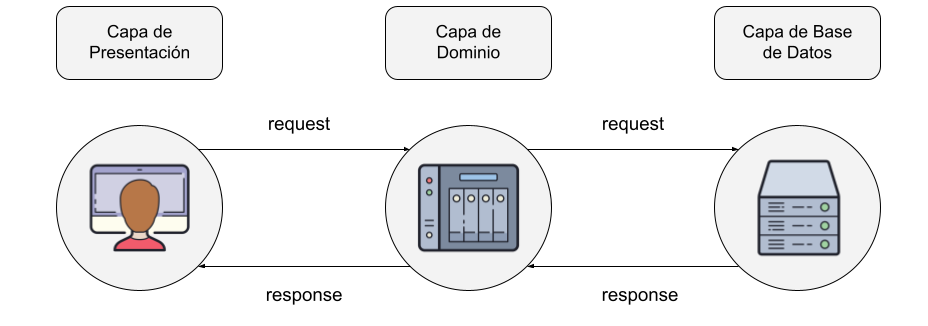
\includegraphics[width=1.03\textwidth]{gfx/Diagrama-arquitectura.png}
    \caption[Diagrama conceptual de la arquitectura]{Diagrama conceptual de la arquitectura.}\label{gfx:Diagrama-arquitectura}
\end{figure}

\section{Capa de Base de Datos}
La capa de base de datos se encarga de las operaciones de los propios datos de la aplicación. Esta capa es invisible para el usuario, ya que su funcionamiento no le incumbe. En esta capa residen los datos y además se acceden a los mismos, mediante solicitudes de almacenamiento o recuperación de información desde la capa de dominio o negocio. Comúnmente esta capa suele pertenecer a la parte Back-end del sistema.

\vspace{0.3cm}

Al tener planteado el \textit{Sprint Backlog} es importante estudiar y analizar las herramientas que compondrán la estructuración de esta capa. Incluso aunque se haya dado ligeras pinceladas de un estudio técnico (\ref{sub:estudio-competitivo-tecnico}), sigue siendo crucial reiterar y volver a incidir en este apartado antes de adentrarse en el diseño de dicha capa.

\subsection{Estudio técnico}
Los dos grandes pilares o modelos que existen actualmente en las bases de datos son denominados SQL (base de datos relacional) y NoSQL (base de datos no relacional). La principal diferencia es que NoSQl no requiere una estructura sólida y definida para trabajar con los datos, lo cual para nuestra aplicación es conveniente ya que requiere de flexibilidad a la hora de operar datos, debido a que estos cambian y se actualizan en un determinado intervalo de tiempo.

\vspace{0.3cm}

Se ha elegido MongoDB como el sistema de base de datos NoSQL, el cual es orientado a documentos y de código abierto. Es de los sistemas más fiables que existen actualmente, además de su conveniencia por ser orientado a objetos, simple, dinámico y escalable. \cite{mongodb-manual}

\vspace{0.3cm}

Se ha elegido el lenguaje Python principalmente por el estudio que se realizó anteriormente en la sección \ref{sub:estudio-competitivo-tecnico}, debido al peso que suponían ambas librerías. Por lo que se ha decidido continuar usando dicho lenguaje y adaptar la base de datos. Pese a que este lenguaje no ha demostrado ser el más eficiente, sigue siendo muy versátil a la hora de trabajar. Con esto, se han seguido las buenas prácticas y se ha usado el \textit{driver} oficial de MongoDB, llamado PyMongo, consiguiendo de manera nativa poder almacenar datos en documentos tipo JSON. Además, Python tiene extensas bibliotecas que procesan directamente los formatos de datos de tipo JSON y BSON. \cite{mongodb-manual}

\vspace{0.3cm}

En cuanto a la plataforma como servicio que se ha elegido en este caso será MongoDB Atlas. Esto debido a que posee un plan gratuito, aunque con muchas limitaciones. La base de datos en la nube funcionaria de la misma manera que en la versión local, pero teniendo en cuenta las limitaciones técnicas.

\vspace{0.3cm}

\begin{figure}[H]
    \centering
    \myfloatalign
    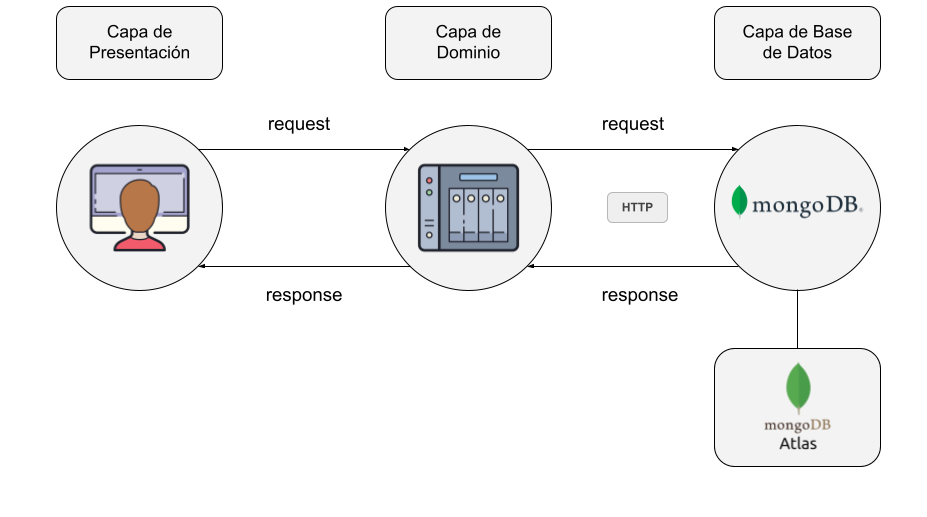
\includegraphics[width=1\textwidth]{gfx/DiagramaRutas1.png}
    \caption[Diagrama conceptual con más detalle (1)]{Diagrama conceptual de la arquitectura, con la Capa de Base de Datos detallada.}\label{gfx:DiagramaRutas1}
\end{figure}

\subsection{Modelado de datos}
El modelo de datos principal será compuesto por dos clases. Las dos clases harán referencia al mismo modelo pero tendrán dos conceptos diferentes, uno para objetos nuevos y otro para su actualización. De esta manera tenemos dos clases, las cuales se llaman \textit{Country} y \textit{CountryUpdate}. La diferencia es que la primera clase creará un id nuevo para cada objeto y la segunda no.

\vspace{0.3cm}

Ambas poseen los mismo atributos y entidades. Están formadas por país y fecha, como los parámetros principales para poder clasificar el objeto y buscarlo en la base de datos. Luego está la lista de diferentes tendencias, la cual se va actualizando a lo largo del día.

\vspace{0.3cm}

Muchos de los atributos pueden llegar a ser opcionales, como por ejemplo la imagen del articulo, la cual si no existe se cargará otra por defecto desde la interfaz. En el siguiente diagrama se puede visualizar el conjunto del modelado, aunque las diferentes entidades serán explicadas en la capa de dominio o negocio.

\vspace{0.3cm}

\begin{figure}[H]
    \centering
    \myfloatalign
    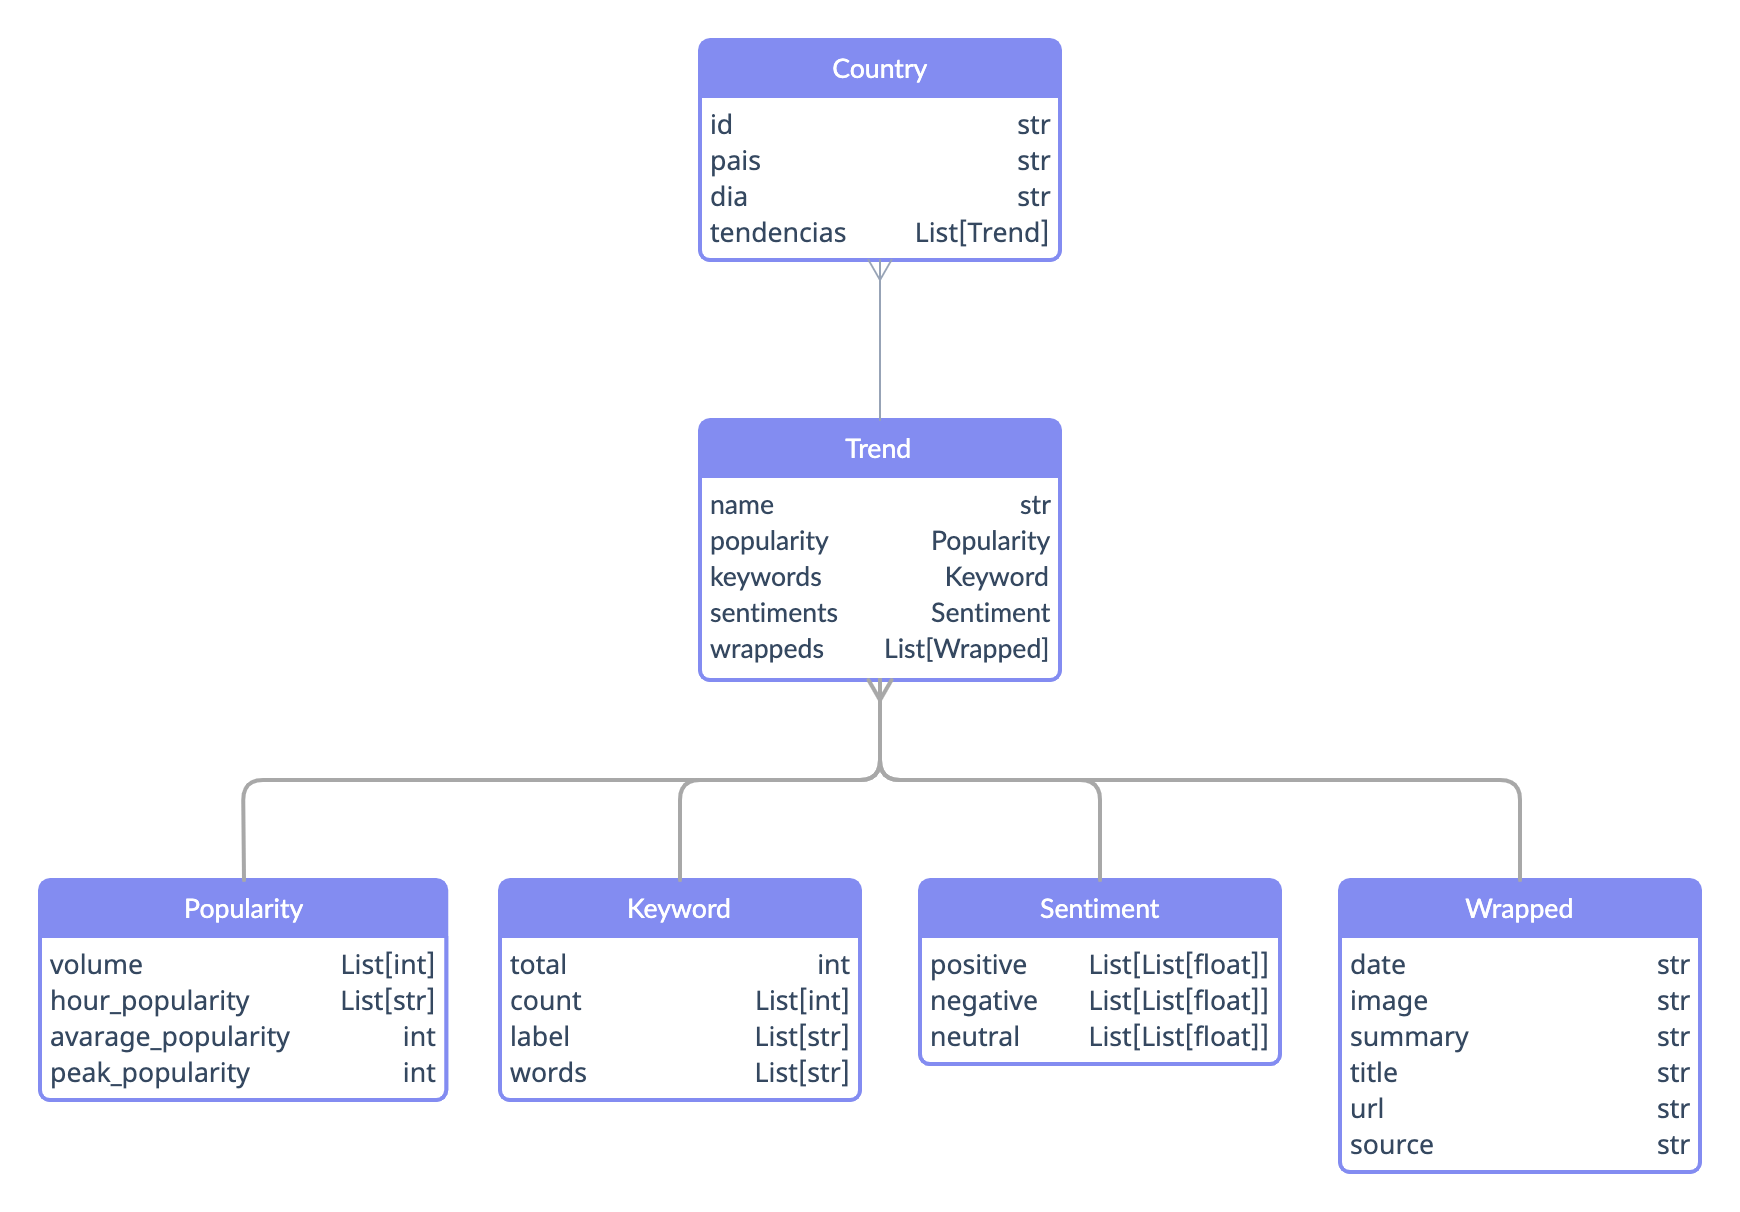
\includegraphics[width=1\textwidth]{gfx/Models-diagram.png}
    \caption[Diagrama de relación de la base de datos]{Diagrama de relación de la base de datos.}\label{gfx:Models-diagram}
\end{figure}

\newpage

\subsubsection{Entidad Tendencia}\label{subsub:ent-tendencia}
Esta entidad representa el modelado de datos de las historias de usuario cubiertas en el Sprint 2 (\ref{subs:sprint-2}). En ellas el usuario debe poder visualizar datos de diez tendencias como máximo.
\begin{figure}[H]
    \centering
    \myfloatalign
    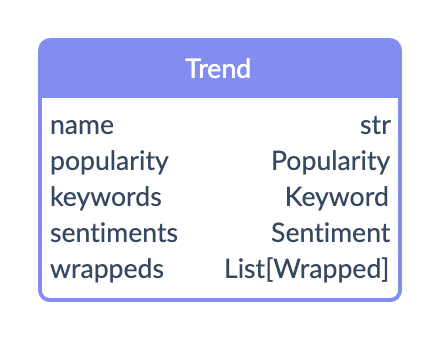
\includegraphics[width=0.4\textwidth]{gfx/diagrama-er0.png}
    \caption[Diagrama de relación de Tendencia]{Diagrama de relación de Tendencia.}\label{gfx:diagrama-er0}
\end{figure}
Para poder representar debidamente la historia de usuario se debe ir calculando progresivamente los siguientes valores:
\\\\
\textit{name}: el nombre de la tendencia.  \\
\textit{popularity}: el objeto popularidad de la tendencia.    \\
\textit{keywords}: el objeto \textit{keywords} de la tendencia.    \\
\textit{sentiments}: el objeto sentimientos general de la tendencia.    \\
\textit{wrappeds}: lista de objetos noticia de la tendencia.

\subsubsection{Entidad Popularidad}\label{subsub:ent-popularidad}
Esta entidad representa el modelado de datos de las historias de usuario cubiertas en el Sprint 6 (\ref{subs:sprint-6}). En ellas el usuario debe poder visualizar datos de interés sobre la popularidad y también una gráfica de área.
\begin{figure}[H]
    \centering
    \myfloatalign
    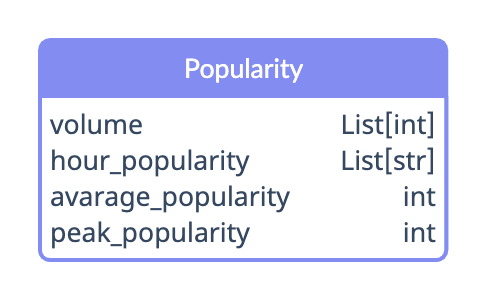
\includegraphics[width=0.4\textwidth]{gfx/diagrama-er1.png}
    \caption[Diagrama de relación de Popularidad]{Diagrama de relación de Popularidad.}\label{gfx:diagrama-er1}
\end{figure}

Para poder representar debidamente las H.U. se debe ir calculando progresivamente los siguientes valores:
\\\\
\textit{volume}: el volumen de popularidad que está teniendo la tendencia.  \\
\textit{hour\_popularity}: la hora en la que fue registrada el volumen.    \\
\textit{avarage\_popularity}: popularidad media de la tendencia.    \\
\textit{peak\_popularity}: popularidad más alta de la tendencia.

\subsubsection{Entidad Palabras más Comunes y Keywords}\label{subsub:ent-keywords}
Esta entidad representa el modelado de datos las historias de usuario cubiertas en el Sprint 7 (\ref{subs:sprint-7}). En ellas el usuario debe poder visualizar datos de interés sobre las palabras más comunes, las \textit{keywords} y una gráfica de radial de barras correspondiente.
\begin{figure}[H]
    \centering
    \myfloatalign
    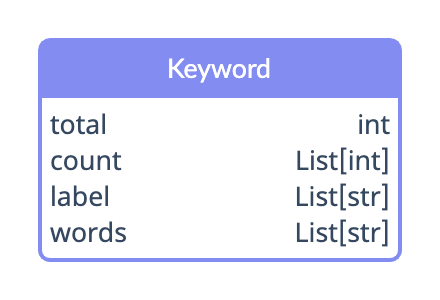
\includegraphics[width=0.4\textwidth]{gfx/diagrama-er2.png}
    \caption[Diagrama de relación de Palabras más Comunes y Keywords]{Diagrama de relación de Palabras más Comunes y Keywords.}\label{gfx:diagrama-er2}
\end{figure}

Para poder representar debidamente las H.U. se debe ir calculando progresivamente los siguientes valores:
\\\\
\textit{total}: el volumen de publicaciones recogidas de la tendencia.  \\
\textit{count}: las repeticiones de palabras comunes.    \\
\textit{label}: las palabras comunes en cuestión.    \\
\textit{words}: las \textit{keywords} extraídas.

\subsubsection{Entidad Sentimiento General}\label{subsub:ent-sentiment}
Esta entidad representa el modelado de datos de las historias de usuario cubiertas en el Sprint 8 (\ref{subs:sprint-8}). En ellas el usuario debe poder visualizar datos de interés sobre el sentimiento general de los tweets o publicaciones y una gráfica de burbujas correspondiente.
\begin{figure}[H]
    \centering
    \myfloatalign
    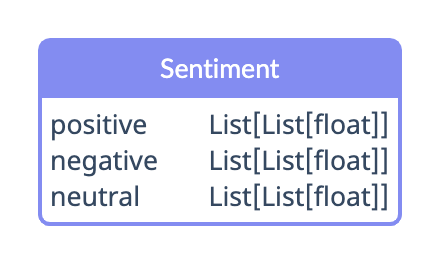
\includegraphics[width=0.4\textwidth]{gfx/diagrama-er3.png}
    \caption[Diagrama de relación de Sentimiento General]{Diagrama de relación de Sentimiento General.}\label{gfx:diagrama-er3}
\end{figure}

Para poder representar debidamente las H.U. se debe ir calculando progresivamente los siguientes valores:
\\\\
\textit{positive}: datos sobre el sentimiento positivo.  \\
\textit{negative}: datos sobre el sentimiento negativo.    \\
\textit{neural}: datos sobre el sentimiento neutro.

\subsubsection{Entidad Noticas Relacionadas}\label{subsub:ent-noticias}
Esta entidad representa el modelado de datos las historias de usuario cubiertas en el Sprint 9 (\ref{subs:sprint-9}). En ellas el usuario debe poder visualizar datos de interés sobre las noticias o artículos relacionados sobre la tendencia.
\begin{figure}[H]
    \centering
    \myfloatalign
    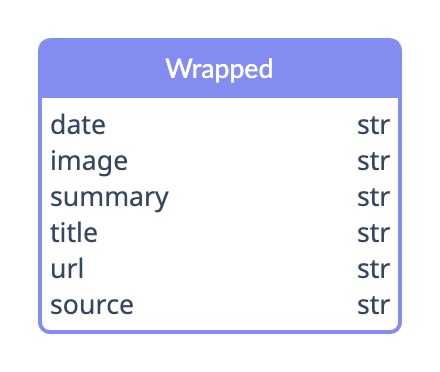
\includegraphics[width=0.4\textwidth]{gfx/diagrama-er4.png}
    \caption[Diagrama de relación de Noticas Relacionadas]{Diagrama de relación de Noticas Relacionadas.}\label{gfx:diagrama-er4}
\end{figure}

Para poder representar debidamente la H.U. se debe ir calculando progresivamente los siguientes valores:
\\\\
\textit{date}: fecha de publicación de la noticia.  \\
\textit{image}: imagen relacionada de la noticia.    \\
\textit{summary}: texto relacionado de la noticia.    \\
\textit{title}: titulo de la noticia.    \\
\textit{url}: enlace de la noticia.    \\
\textit{source}: editorial de la noticia.

\section{Capa de Dominio o Negocio}
La capa de dominio o negocio permite la interacción entre la capa de base de datos y la capa de presentación. Es la capa encargada de gestionar tanto las distintas peticiones recibidas desde la capa de presentación, como los datos almacenados en la capa de base de datos. Comúnmente esta capa suele pertenecer a la parte Back-end del sistema.

\subsection{Estudio técnico}
Al plantear la aplicación en la capa de dominio o negocio, surgen ciertas pautas o normativas que conviene seguir. Surge la denominación \ac{API} para las interacciones que surgen entre la capa de presentación y la capa actual. Otra denominación que conviene saber es \ac{REST}, el cual es un conjunto de limites a la hora de implementar una \ac{API}. \cite{redahat-manual}

\vspace{0.3cm}

Cuando un usuario envía una petición a través de una API REST o RESTful, esta transfiere una representación del estado del recurso solicitado al solicitante o al extremo. Generalmente la información se envía a través de \ac{HTTP} en formato \ac{JSON}, un lenguaje popular y fácilmente entendible. \cite{redahat-manual}

\vspace{0.3cm}

La mayoría de las interacciones se pueden resumir en el nemónico de las cuatro funciones del almacenamiento persistente llamado \ac{CRUD}. Las funciones \ac{CRUD} implican el uso de las operaciones \ac{HTTP}, las cuales son PUT, GET, POST, DELETE o PATCH.

\vspace{0.3cm}

Habiendo definido propiamente las pautas de una \ac{API} \ac{REST}, podemos proceder a elegir el \textit{microframework} que cumpla y revele las operaciones salientes mediante la interfaz \ac{REST} y \textit{websockets}. Para ello se ha elegido de nuevo el lenguaje Python, debido a que exista compatibilidad entre la capa de base de datos y la de dominio o negocio y además por su versatilidad a la hora de trabajar con diferentes librerías que  serán extremadamente útiles para la realización de diversas historias de usuario.

\vspace{0.3cm}

Actualmente, en Python existen \textit{frameworks} que funcionan con el estándar \ac{WSGI} o \ac{ASGI}. El último mencionado es el más actual y utiliza corrutinas introducidas en las versiones más recientes de Python, lo que mejora el uso de la CPU en servidores web intensivos de E/S.

\vspace{0.3cm}

Las principales implementaciones de servidor \ac{ASGI} existentes actuales son Uvicorn, Hypercorn y Daphne. Los tres son fácilmente implementables, pero el más estable es Uvicorn, además usa una implementación escrita directamente en el lenguaje C, lo cual lo vuelve más rápido y eficiente. \cite{uvicorn-manual}

\vspace{0.3cm}

Tras haber elegido el servidor, podemos continuar con el \textit{microframework}. Actualmente existe una cantidad variada de ellos, como FastAPI, Starlette o Django, pero finalmente me he decantado por la primera opción. FastAPI es mucho más ligero que Django y además funciona de una manera parecida a Starlette, pero le añade funcionalidades como validación o documentación. \cite{fastapi-manual}

\vspace{0.3cm}

La implementación de las rutas fue realizada con el objeto \textit{router}, el cual tiene la función de declarar todas las rutas con decoradores y añadir el prefijo que llevaran dichas rutas. Posteriormente se crea la documentación automática.

\vspace{0.3cm}

\begin{figure}[H]
    \centering
    \myfloatalign
    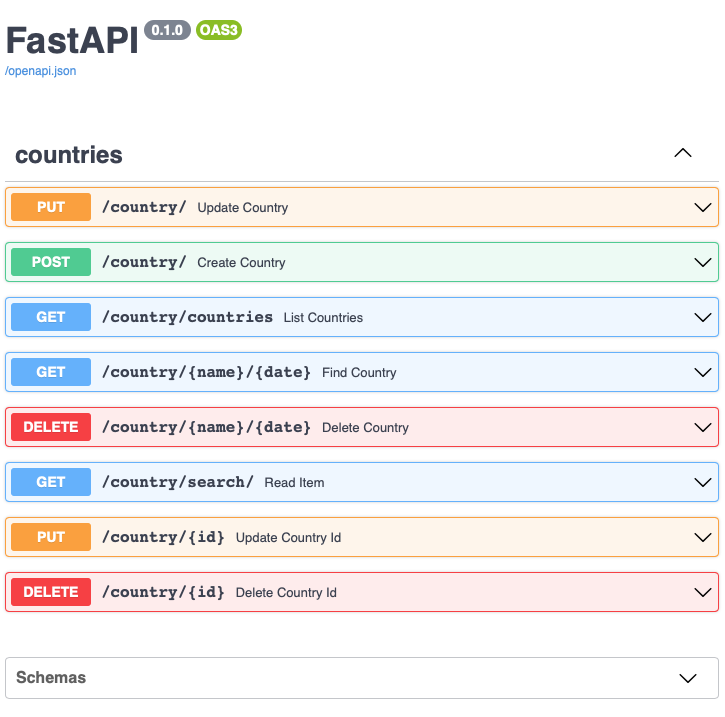
\includegraphics[width=1\textwidth]{gfx/fastapi-rutas.png}
    \caption[Documentación generada por FastAPI]{Documentación generada por FastAPI.}\label{gfx:fastapi-rutas}
\end{figure}

En cuanto a la plataforma como servicio (\ac{PaaS}) he elegido Heroku, la cual tiene opciones gratuitas y está basada en contenedores. La gran ventaja de Heroku, aparte de tener un plan gratuito, es que tiene múltiple soporte de lenguajes y entre ellos Python. Las rutas declaradas y la de por defecto funcionarían de la misma manera que localmente. \cite{heroku-manual}

\vspace{0.3cm}

Además otra ventaja crucial, la cual es requerida para el correcto funcionamiento de la aplicación, es que un proceso se ejecute cada determinado intervalo de tiempo. Esto es debido a que necesitamos que se actualice la información de las tendencias, por lo que localmente tendríamos que configurar un \textit{cron} ejecutando un \textit{script} de Python y en Heroku tenemos un \textit{Scheduler}, el cual tiene el mismo comportamiento. Dicho proceso ha sido configurado para que se ejecute cada hora y el \textit{script} en cuestión recopilará toda la información necesaria.

\vspace{0.3cm}

\begin{figure}[H]
    \centering
    \myfloatalign
    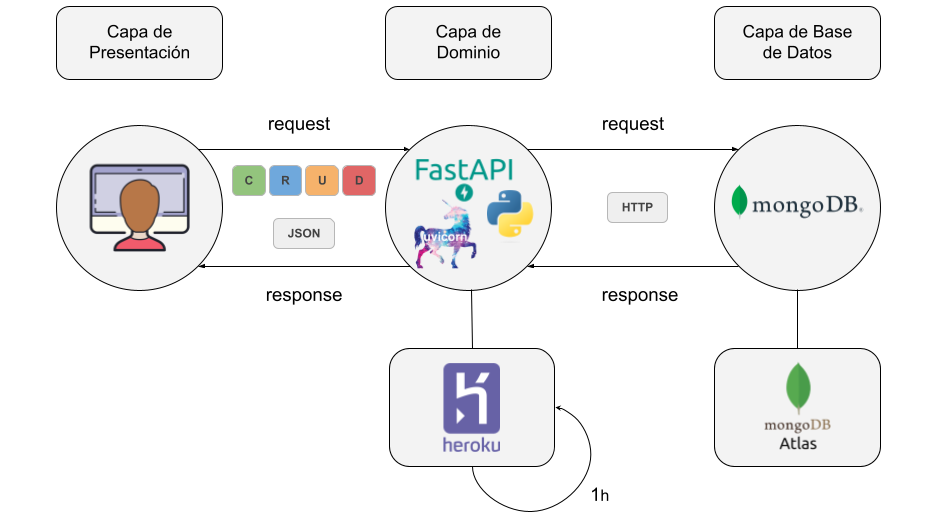
\includegraphics[width=0.91\textwidth]{gfx/DiagramaRutas2.png}
    \caption[Diagrama conceptual con más detalle (2)]{Diagrama conceptual de la arquitectura, con la Capa de Dominio o Negocio y Base de Datos detallada.}\label{gfx:DiagramaRutas2}
\end{figure}

\subsection{Diagramas de interacción de distintas rutas}

\begin{figure}[H]
    \centering
    \myfloatalign
    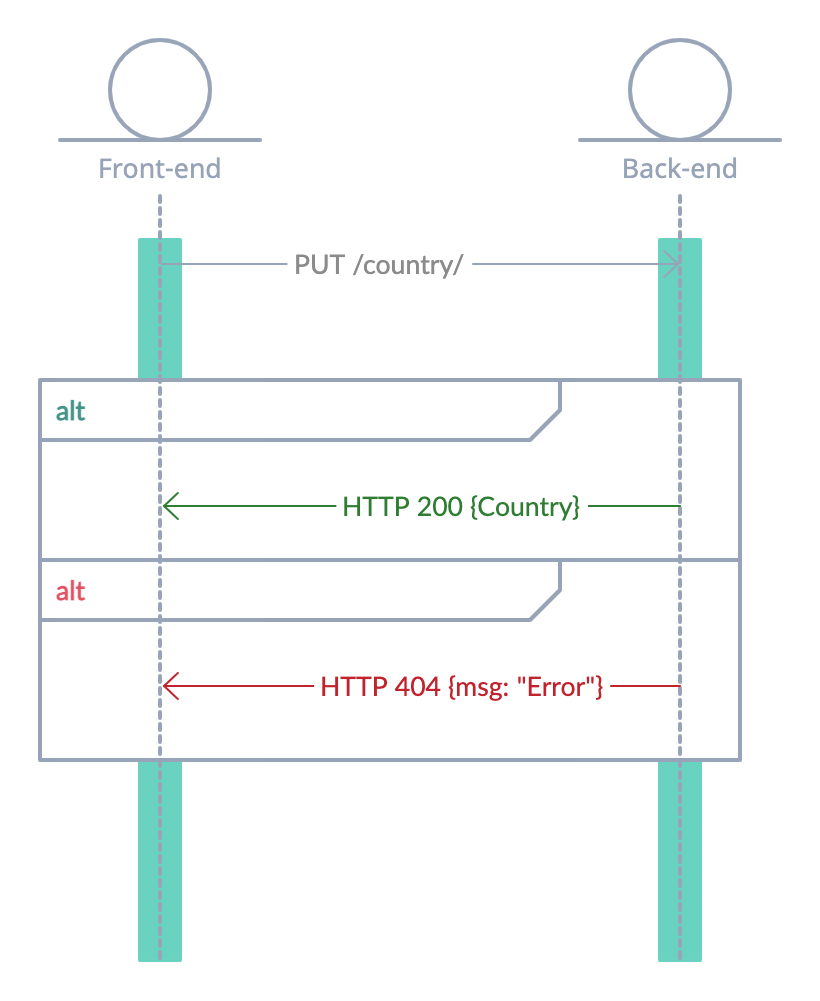
\includegraphics[width=0.39\textwidth]{gfx/diagrama-itr1.png}
    \caption[Diagrama interacción de rutas (1)]{Diagrama interacción de rutas: \textit{Actualización de Country}.}\label{gfx:diagrama-itr1}
\end{figure}

\begin{figure}[H]
    \centering
    \myfloatalign
    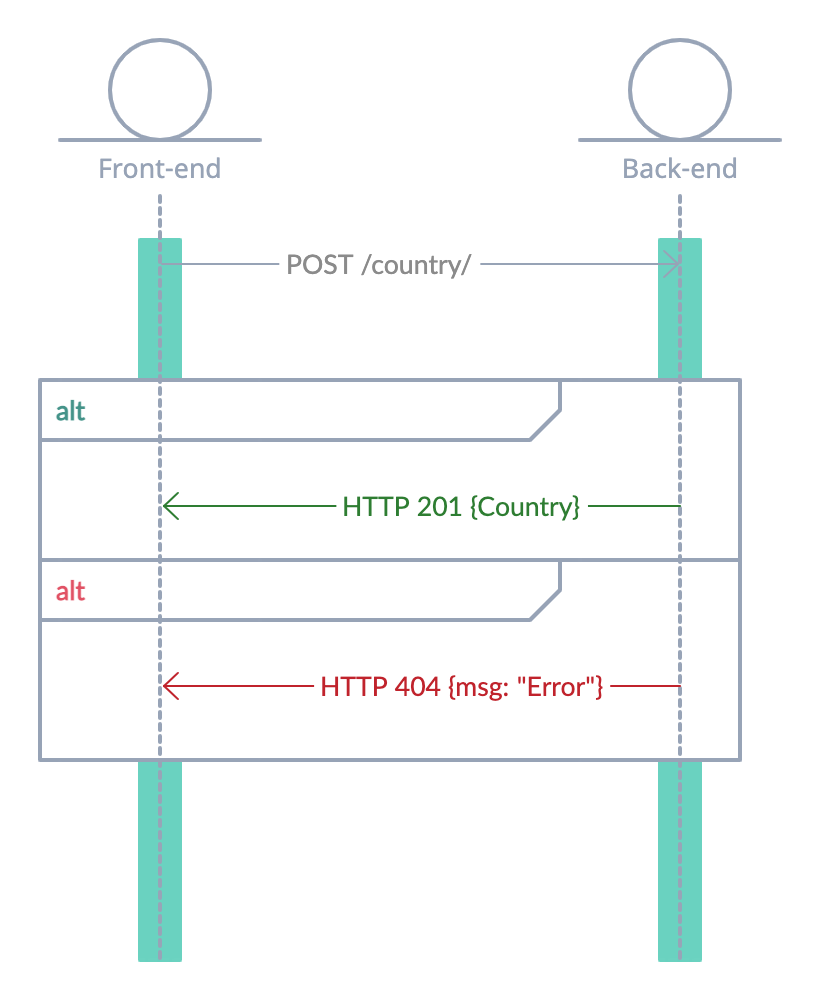
\includegraphics[width=0.39\textwidth]{gfx/diagrama-itr2.png}
    \caption[Diagrama interacción de rutas (2)]{Diagrama interacción de rutas: \textit{Creación de Country}.}\label{gfx:diagrama-itr2}
\end{figure}

\begin{figure}[H]
    \centering
    \myfloatalign
    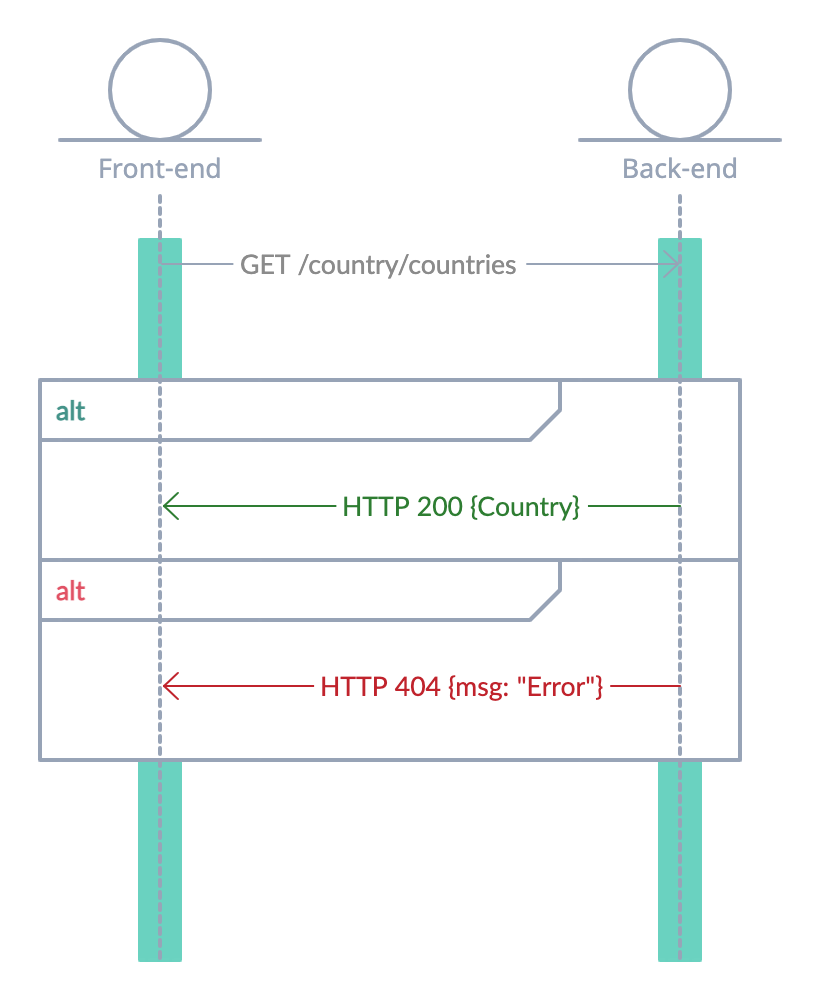
\includegraphics[width=0.44\textwidth]{gfx/diagrama-itr3.png}
    \caption[Diagrama interacción de rutas (3)]{Diagrama interacción de rutas: \textit{Lectura de lista de Country}.}\label{gfx:diagrama-itr3}
\end{figure}

\begin{figure}[H]
    \centering
    \myfloatalign
    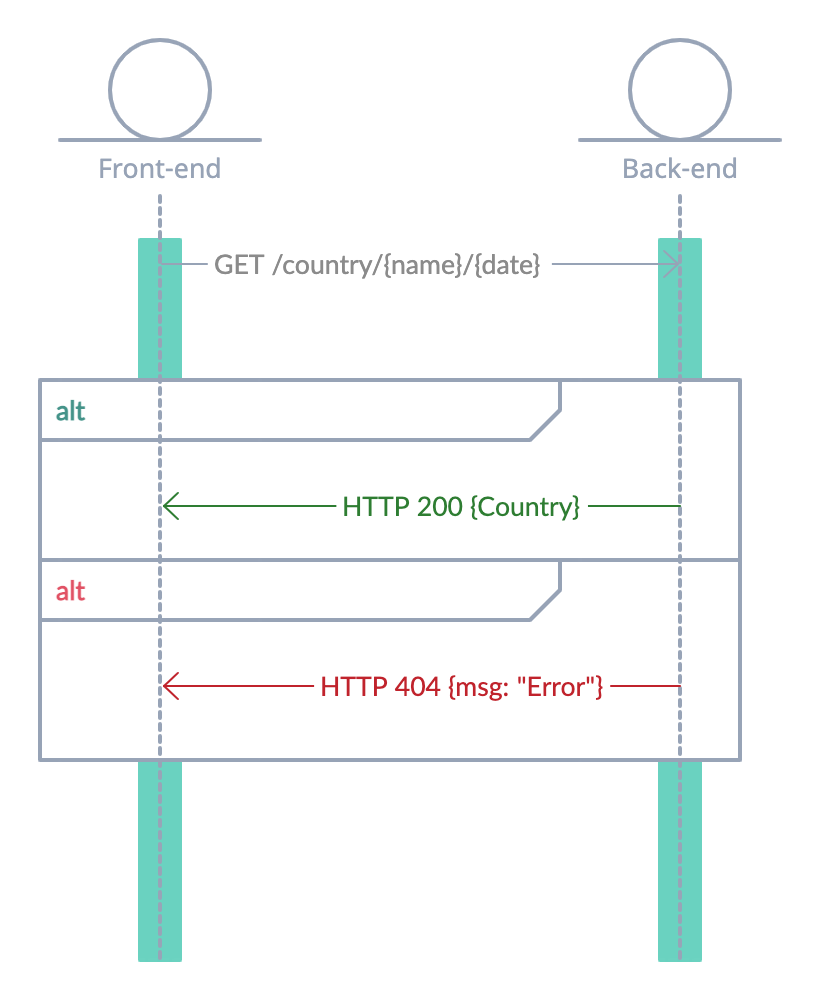
\includegraphics[width=0.44\textwidth]{gfx/diagrama-itr4.png}
    \caption[Diagrama interacción de rutas (4)]{Diagrama interacción de rutas: \textit{Lectura de Country por parámetros}.}\label{gfx:diagrama-itr4}
\end{figure}

\begin{figure}[H]
    \centering
    \myfloatalign
    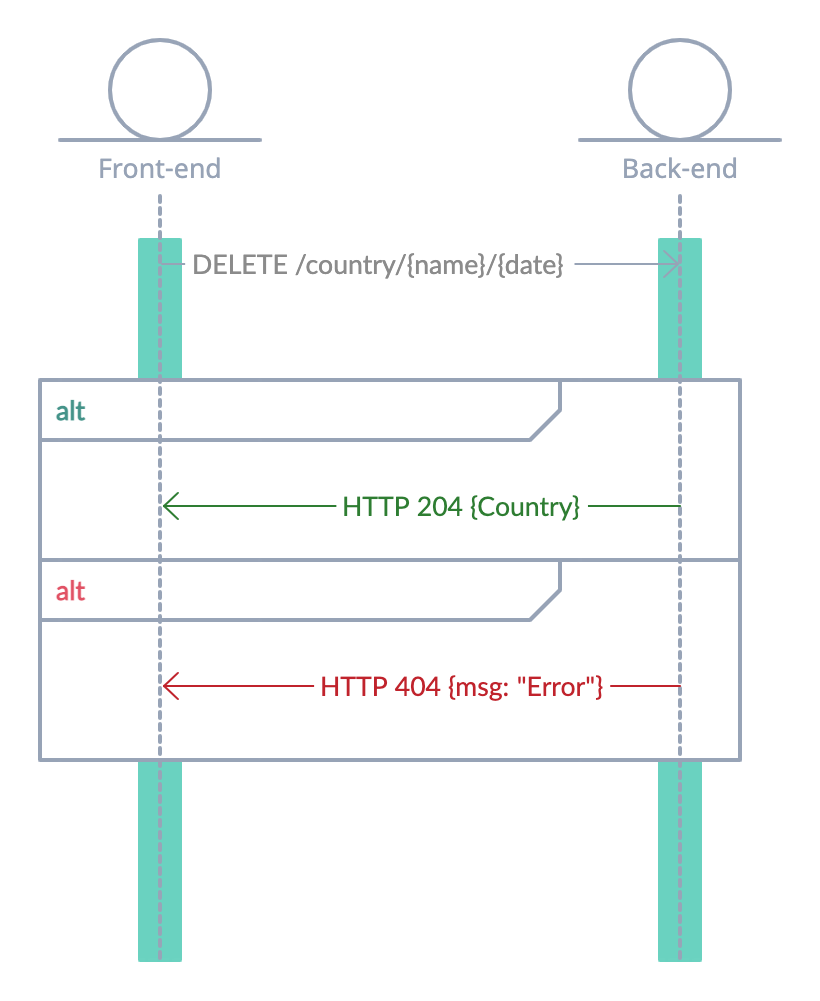
\includegraphics[width=0.44\textwidth]{gfx/diagrama-itr5.png}
    \caption[Diagrama interacción de rutas (5)]{Diagrama interacción de rutas: \textit{Eliminación de Country por parámetros}.}\label{gfx:diagrama-itr5}
\end{figure}

\begin{figure}[H]
    \centering
    \myfloatalign
    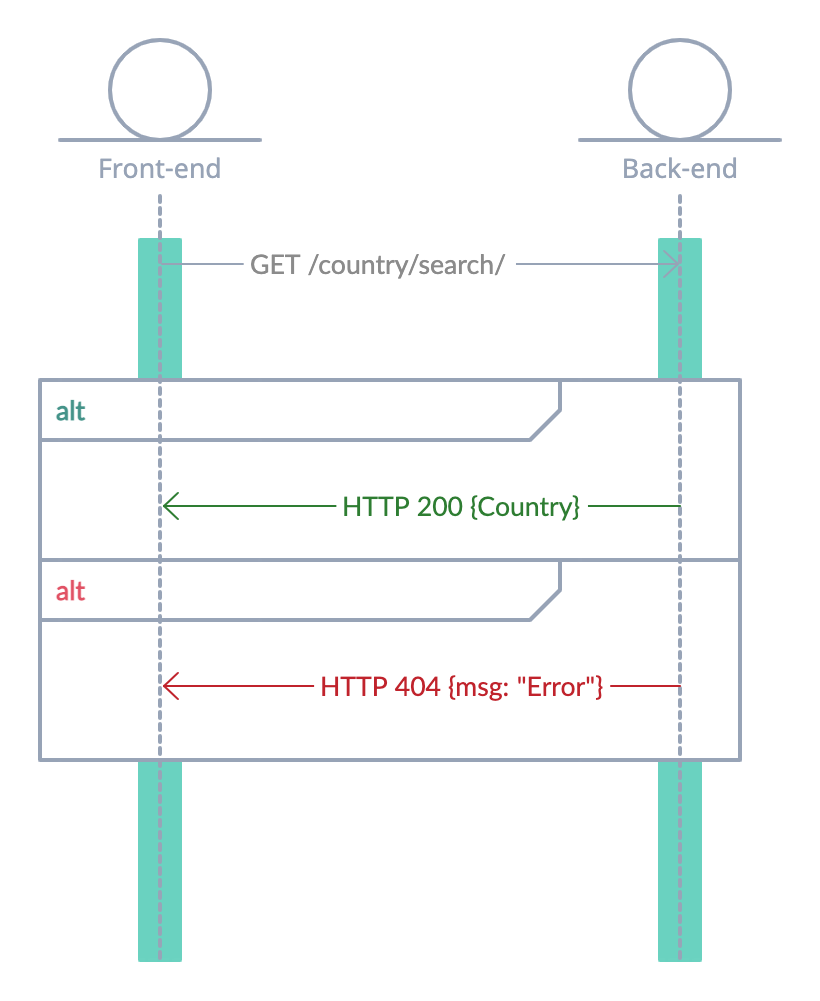
\includegraphics[width=0.45\textwidth]{gfx/diagrama-itr6.png}
    \caption[Diagrama interacción de rutas (6)]{Diagrama interacción de rutas: \textit{Lectura de la búsqueda de Country}.}\label{gfx:diagrama-itr6}
\end{figure}

\begin{figure}[H]
    \centering
    \myfloatalign
    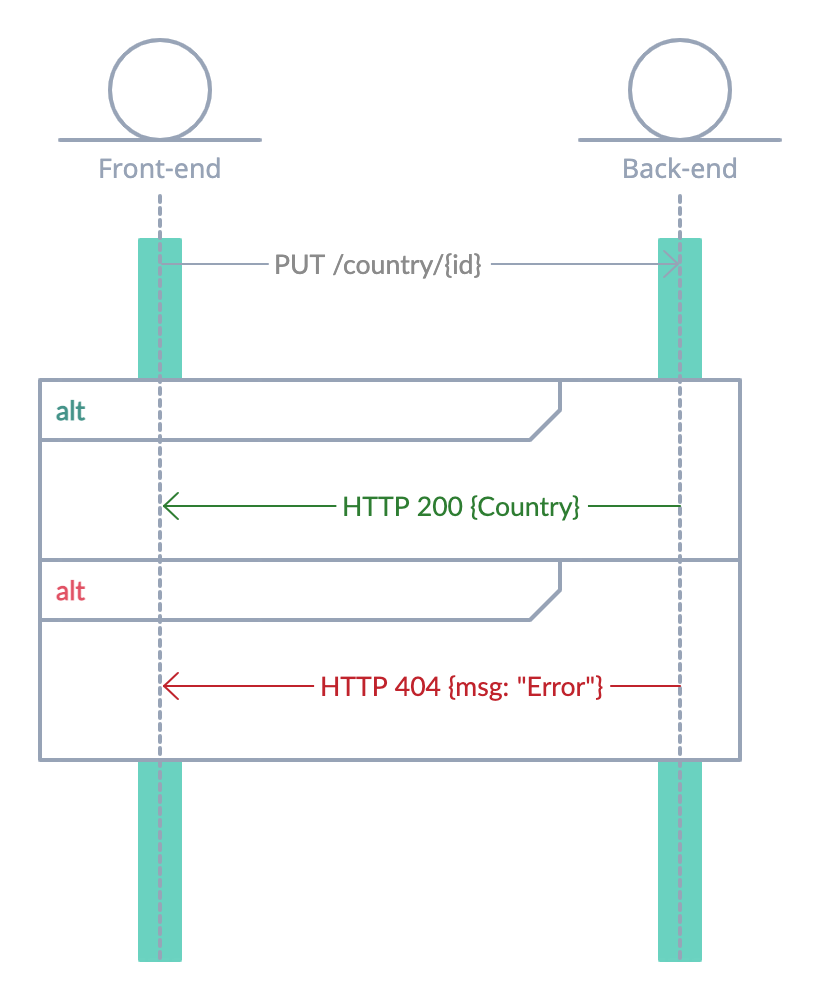
\includegraphics[width=0.45\textwidth]{gfx/diagrama-itr7.png}
    \caption[Diagrama interacción de rutas (7)]{Diagrama interacción de rutas: \textit{Actualización de Country por id}.}\label{gfx:diagrama-itr7}
\end{figure}

\begin{figure}[H]
    \centering
    \myfloatalign
    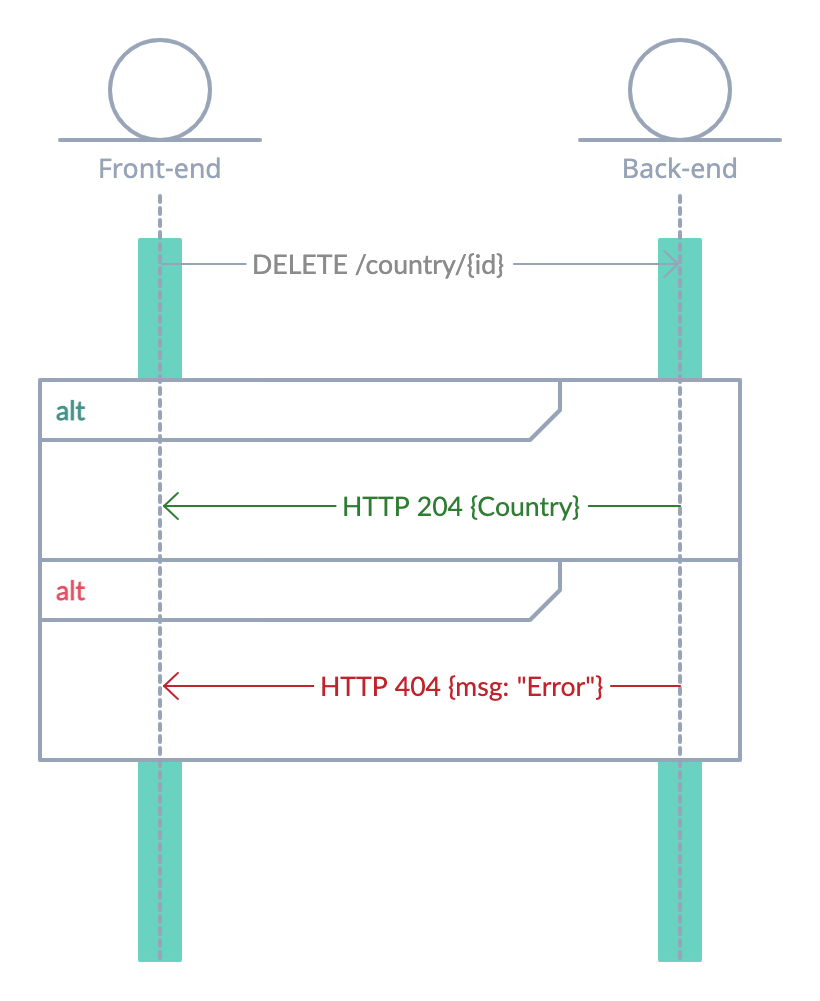
\includegraphics[width=0.45\textwidth]{gfx/diagrama-itr8.png}
    \caption[Diagrama interacción de rutas (8)]{Diagrama interacción de rutas: \textit{Eliminación de Country por id}.}\label{gfx:diagrama-itr8}
\end{figure}

\section{Capa de Presentación}
La capa de presentación se encarga de visualizar el contenido de la aplicación, donde el usuario puede interactuar directamente. De este modo esta capa será la única visible para el usuario. Comúnmente esta capa se suele denominar como Front-end.

\subsection{Estudio técnico}
Al buscar el \textit{framework} idóneo para la visualización de la aplicación surgen muchas posibilidades. Una entre ellas fue Vue, esta opción destaca por su rendimiento, escalabilidad y buena documentación. A la vez es mucho más ligera que sus competidores y además ofreciendo las mismas características, como por ejemplo el uso del \ac{DOM} virtual, el cual tiene sus ventajas a la hora de renderizar los mismos componentes de una página. En nuestro caso los componentes como las cartas se podrían beneficiar de ello. \cite{VueComparison}

\vspace{0.3cm}

Uno de los principales objetivos de la aplicación, que ya se había planteado antes, es que el contenido se pueda visualizar por medio de módulos o cartas. Por lo que al diseñar la propia aplicación, tendremos una vista principal y cada una de las cartas estará dividida en una subvista. Cada subvista tendrá sus propiedades, sus propias funciones y clases CSS. La mayoría de las clases estarán implementadas directamente a mano, menos las más básicas o convenientes ya que usaré el \textit{framework} TailwindCSS para agilizar el trabajo.

\vspace{0.3cm}

En cuanto a la plataforma como servicio (\ac{PaaS}) para la capa de presentación me he decantado por Vercel, realmente tenía mucho parecido a otras plataformas como Netlify, aunque tras usar ambas plataformas he podido concluir que Vercel funciona más eficientemente y de una manera más simple. Además posee integración con Vue, lo cual me ha permitido exportar fácilmente el proyecto.

\begin{figure}[H]
    \centering
    \myfloatalign
    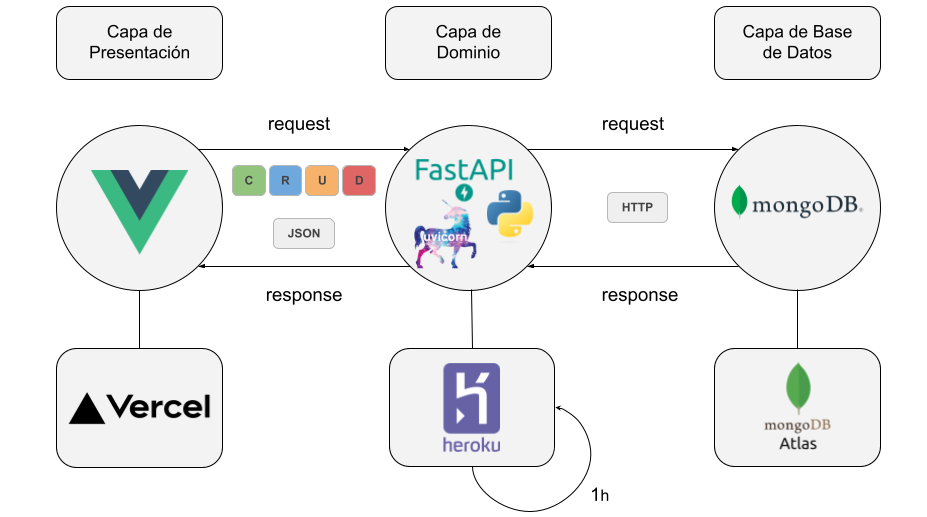
\includegraphics[width=0.83\textwidth]{gfx/DiagramaRutas3.png}
    \caption[Diagrama conceptual con más detalle (3)]{Diagrama conceptual de la arquitectura, con la Capa de Dominio o Negocio, Base de Datos y Presentación detallada.}\label{gfx:DiagramaRutas3}
\end{figure}

El contenido de la vista principal se adapta mediante parámetros y rutas. Aunque existan diferentes rutas en la capa de presentación, todas ellas devuelven la misma vista principal con los mismos componentes, a no ser que haya un error. En el siguiente diagrama se explica el funcionamiento de las distintas rutas, tanto la ruta por defecto, la ruta de la búsqueda de un tópico o la ruta por parámetros.

\begin{itemize}
    \item
    \textit{Ejemplo de ruta por defecto: \\
    https://(...)/}
    \item
    \textit{Ejemplo de ruta de búsqueda: \\
    https://(...)/search?name=Spain\&query=baloncesto}
    \item
    \textit{Ejemplo de ruta por parámetros: \\
    https://(...)/Spain/22-10-24}
\end{itemize}

\begin{figure}[H]
    \centering
    \myfloatalign
    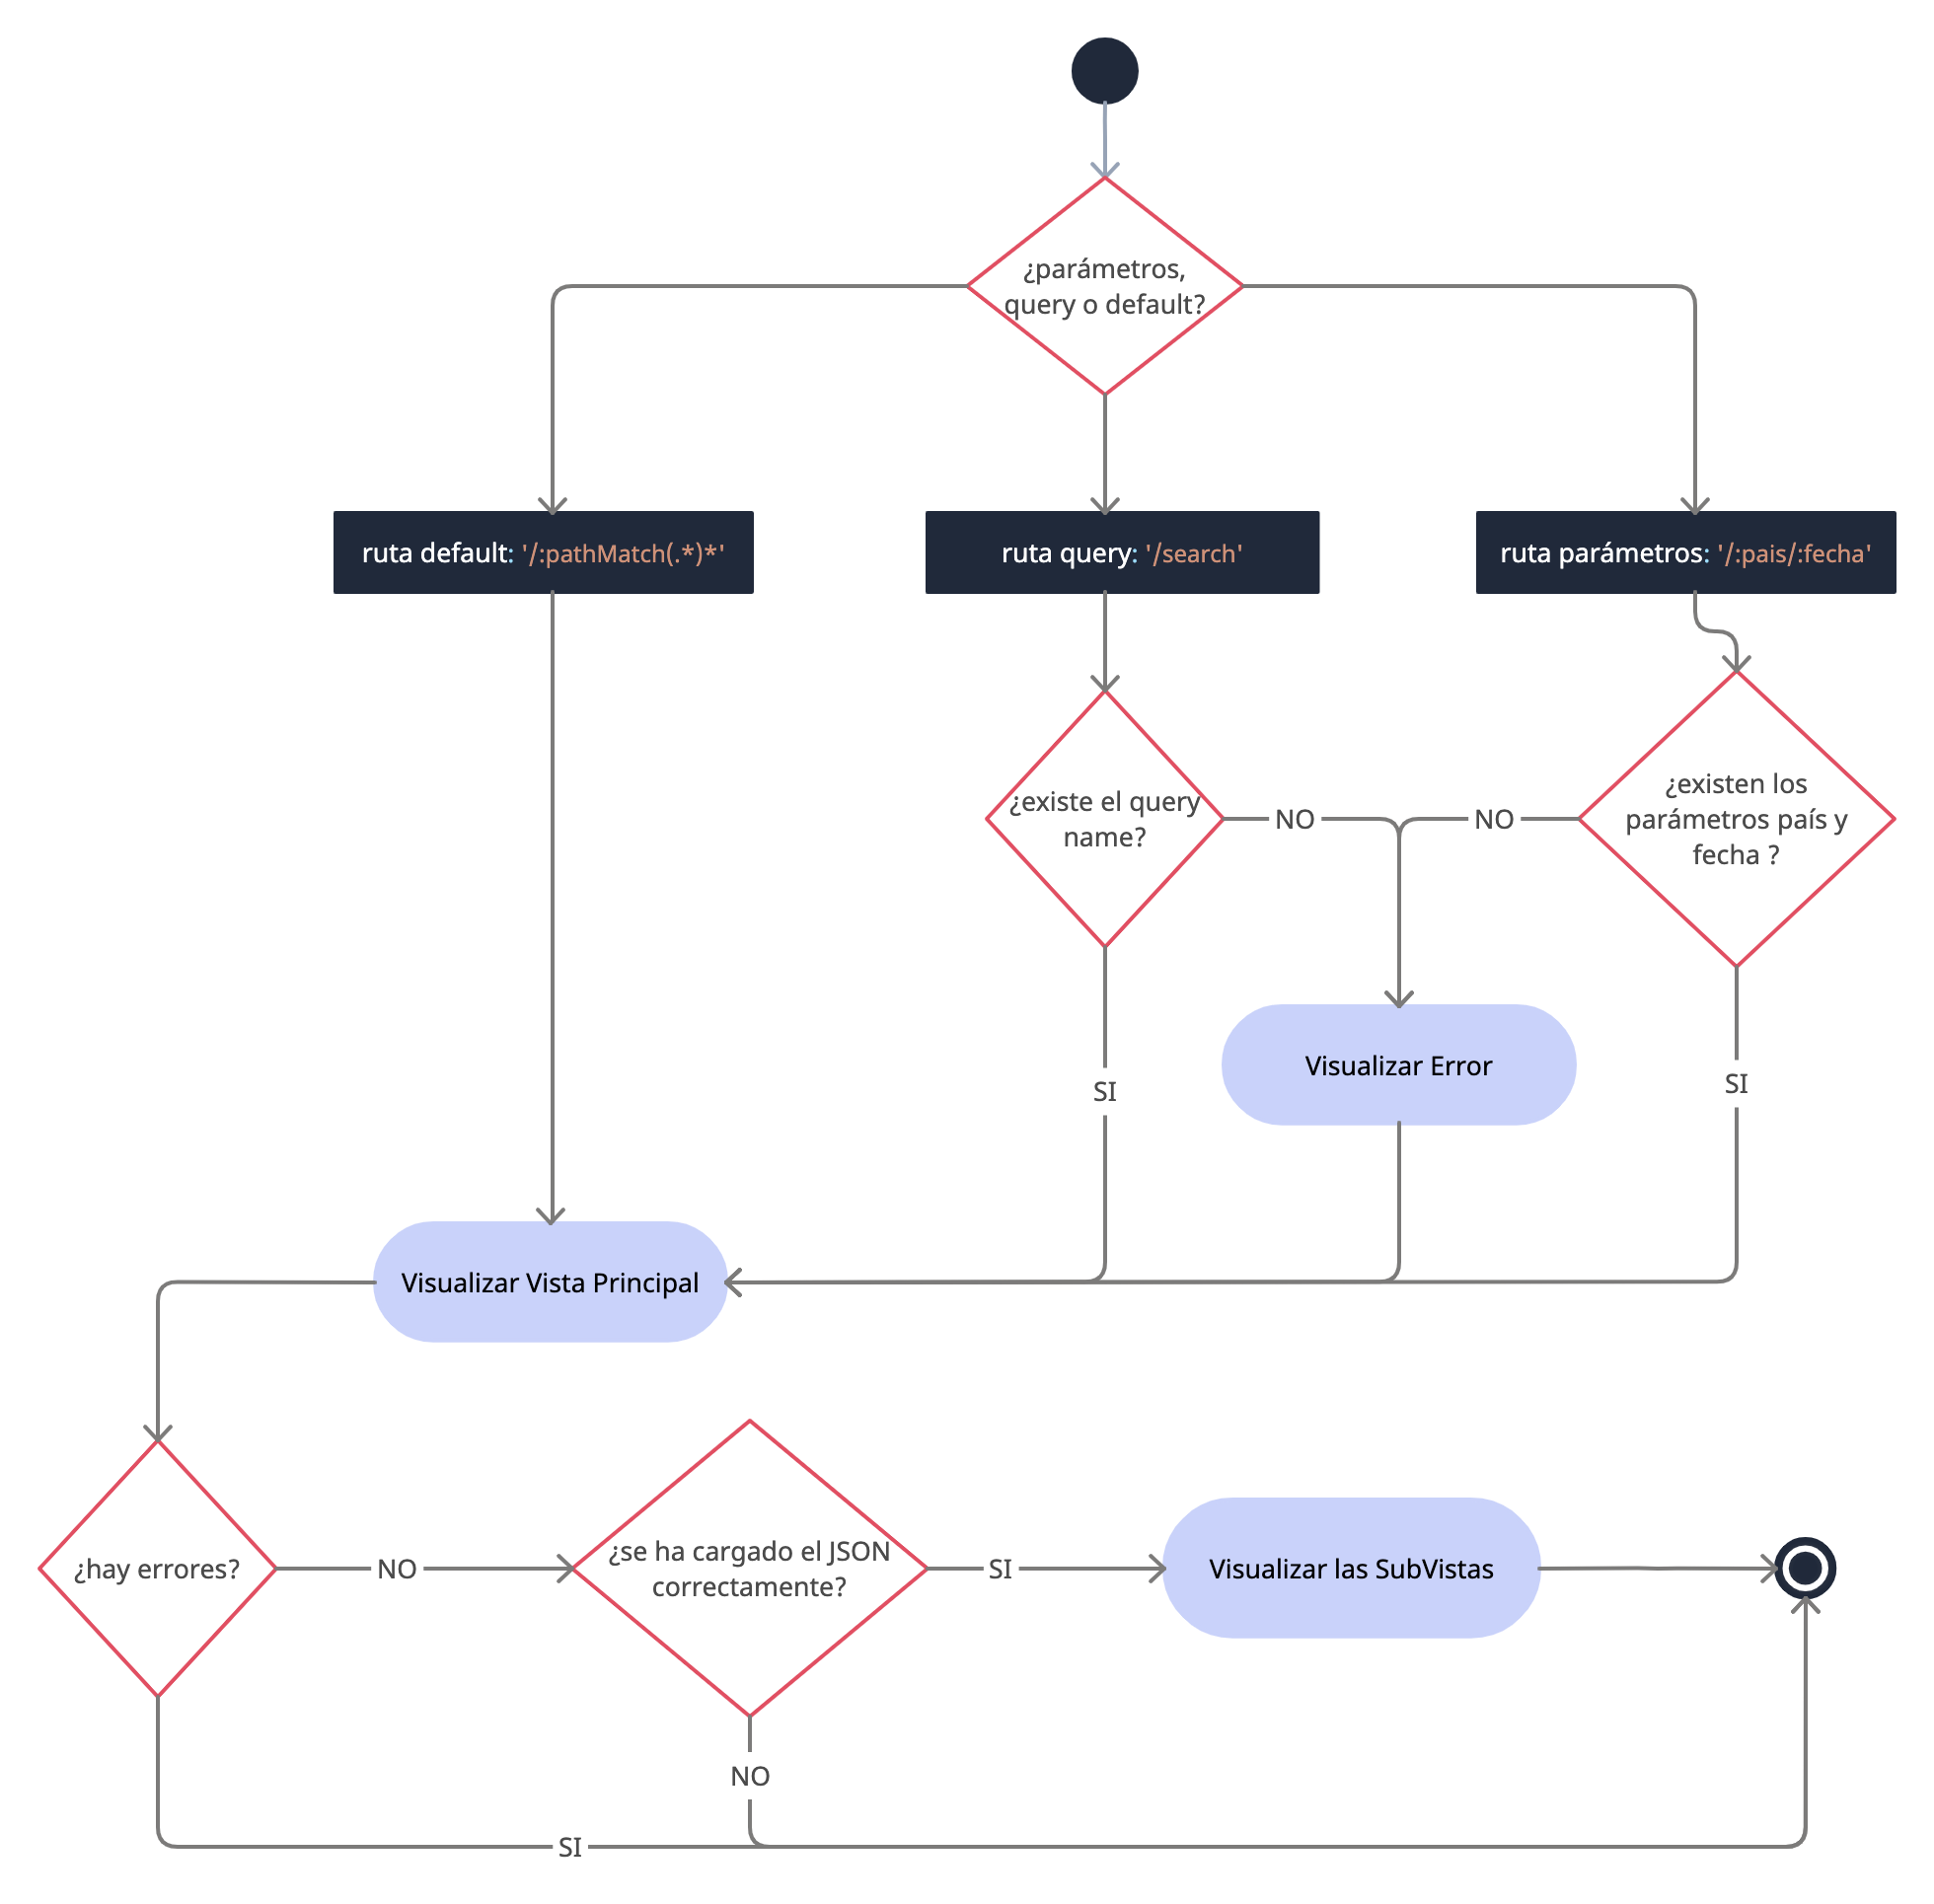
\includegraphics[width=1.001\textwidth]{gfx/Diagrama-actividad.png}
    \caption[Diagrama de actividad]{Diagrama de actividad.}\label{gfx:Diagrama-actividad}
\end{figure}

La ruta por defecto cargará como parámetro el país España y la fecha del día actual. Las demás rutas son ejecutadas al interactuar con los componentes de distintos formularios de la página. En este caso son dos, un formulario de selección (fecha y país) y otro formulario de búsqueda (los tópicos).

\vspace{0.3cm}

\begin{figure}[H]
    \centering
    \myfloatalign
    
\includegraphics[width=0.9\textwidth]{gfx/Formularios.png}
    \caption[Formularios de selección y búsqueda]{Formularios de selección y búsqueda.}\label{gfx:Formularios}
\end{figure}

Cada uno funcionan de una manera independiente, mediante eventos por click. Aunque si precisan de la información que hay en cada formulario, es decir, si el usuario cambia el parámetro país, entonces se carga una ruta con la fecha y el país seleccionado. Esto ocurre de la misma manera seleccionando la fecha o buscando un tópico, ambos necesitan la información del país seleccionado para procesar la ruta.

\subsection{Transcurso de la Interfaz de Usuario}
La vista principal es la única vista que se le llega mostrar al usuario, por lo que es importante mostrar el transcurso que ha tenido su propio diseño. Aunque como hemos explicado la vista principal se subidivide y cada subvista tiene sus propias clases de CSS, en español «Hojas de estilo en cascada». Cabe mencionar, que también se ha empleado una biblioteca que fue crucial llamada TailwindCSS.

\begin{figure}[H]
    \centering
    \myfloatalign
    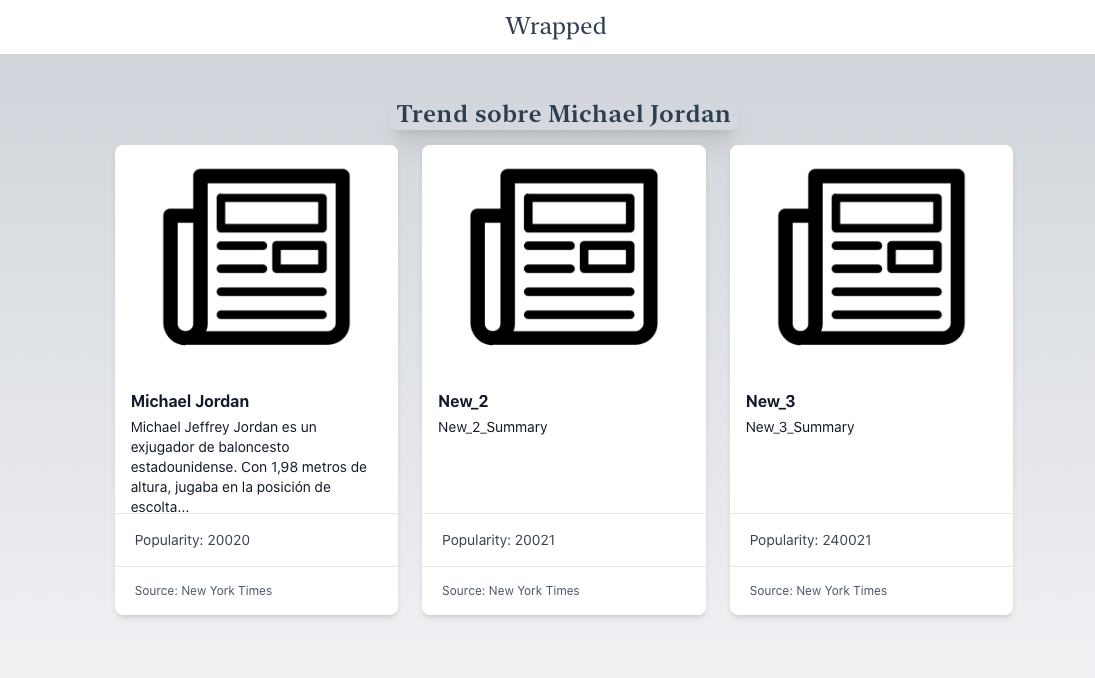
\includegraphics[width=1\textwidth]{gfx/primer-boceto.png}
    \caption[Primer boceto de la aplicación]{Primer boceto de la aplicación.}\label{gfx:primer-boceto}
\end{figure}

\begin{figure}[H]
    \centering
    \myfloatalign
    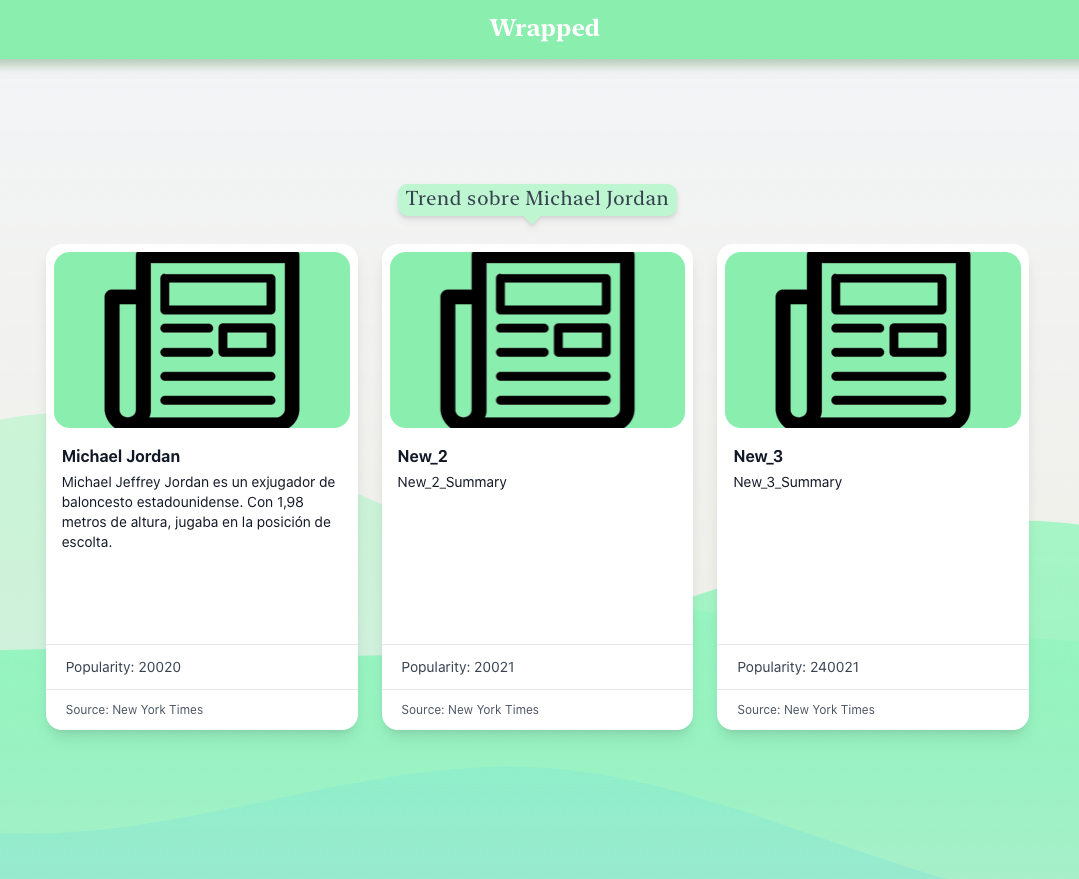
\includegraphics[width=1\textwidth]{gfx/segundo-boceto.png}
    \caption[Segundo boceto más detallado]{Segundo boceto más detallado.}\label{gfx:segundo-boceto}
\end{figure}

\begin{figure}[H]
    \centering
    \myfloatalign
    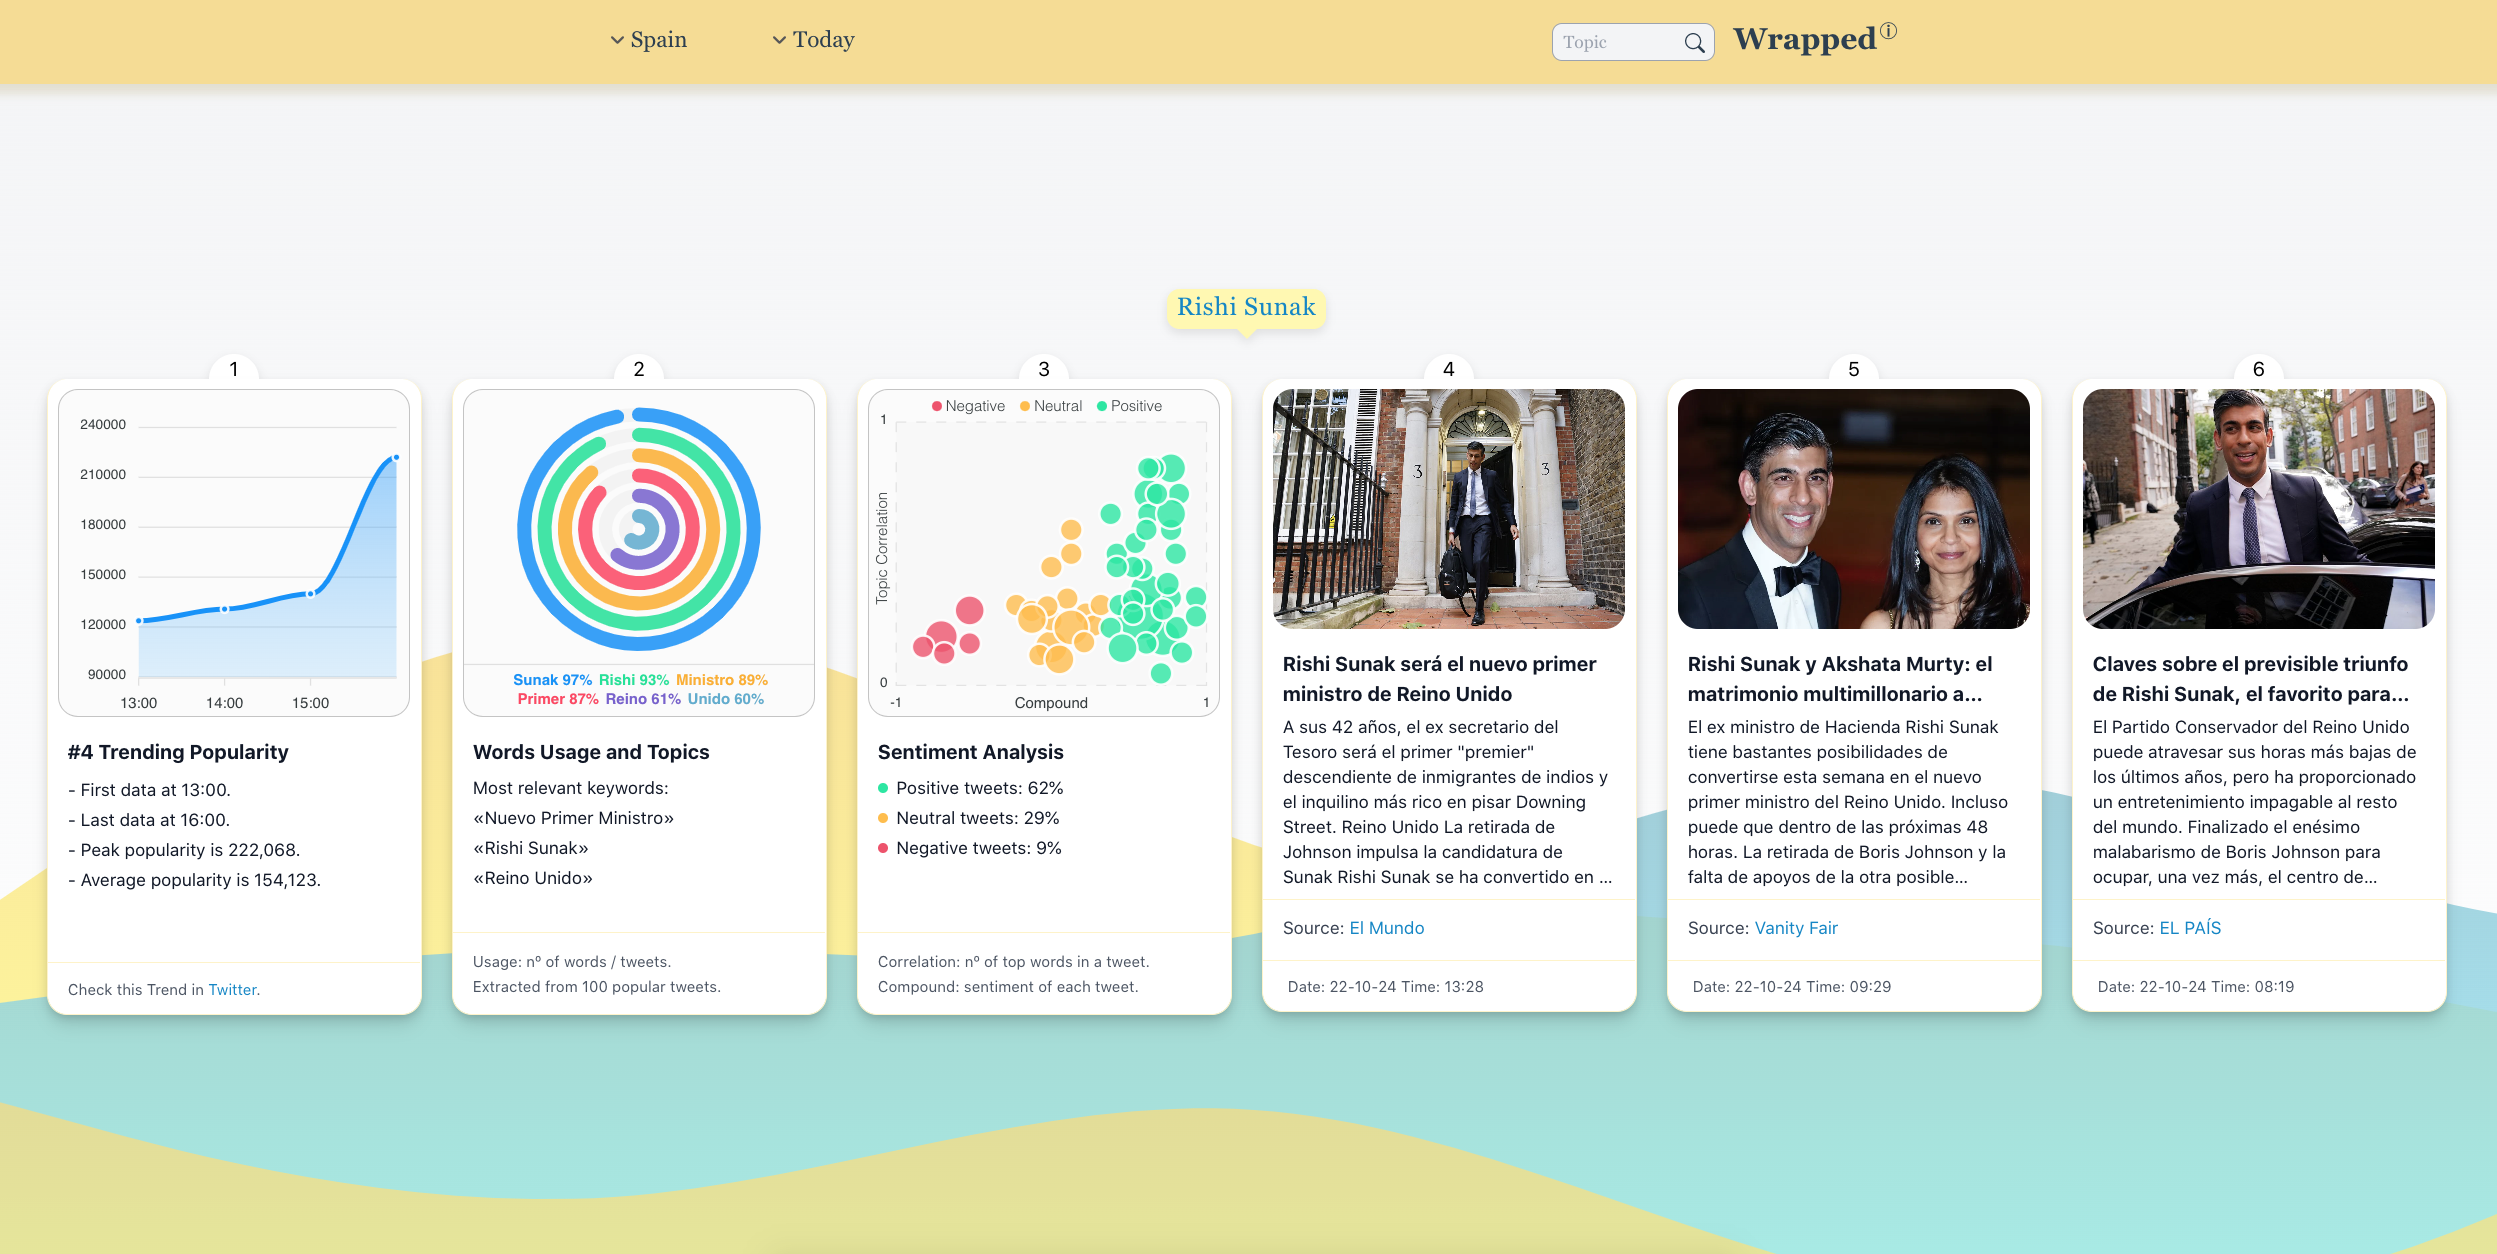
\includegraphics[width=1\textwidth]{gfx/tercer-boceto.png}
    \caption[Concepto final de la aplicación]{Concepto final de la aplicación.}\label{gfx:tercer-boceto}
\end{figure}

\begin{figure}[H]
    \centering
    \myfloatalign
    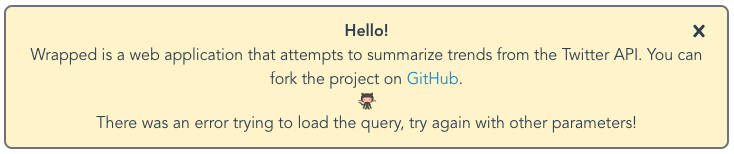
\includegraphics[width=1\textwidth]{gfx/boceto-error.png}
    \caption[Concepto del error en la visualización de parámetros]{Concepto del error en la visualización de parámetros.}\label{gfx:boceto-error}
\end{figure}

\subsection{Vista Principal}
La vista principal contiene todas las subvistas y componentes necesarios para el funcionamiento de la interfaz. Cada subvista funciona como un componente esencial dentro de la vista principal. Al cargar correctamente los datos desde la capa de dominio o negocio, estos se representan en la vista principal y a la vez cada entidad se representa con una subvista diferente.

\begin{figure}[H]
    \centering
    \myfloatalign
    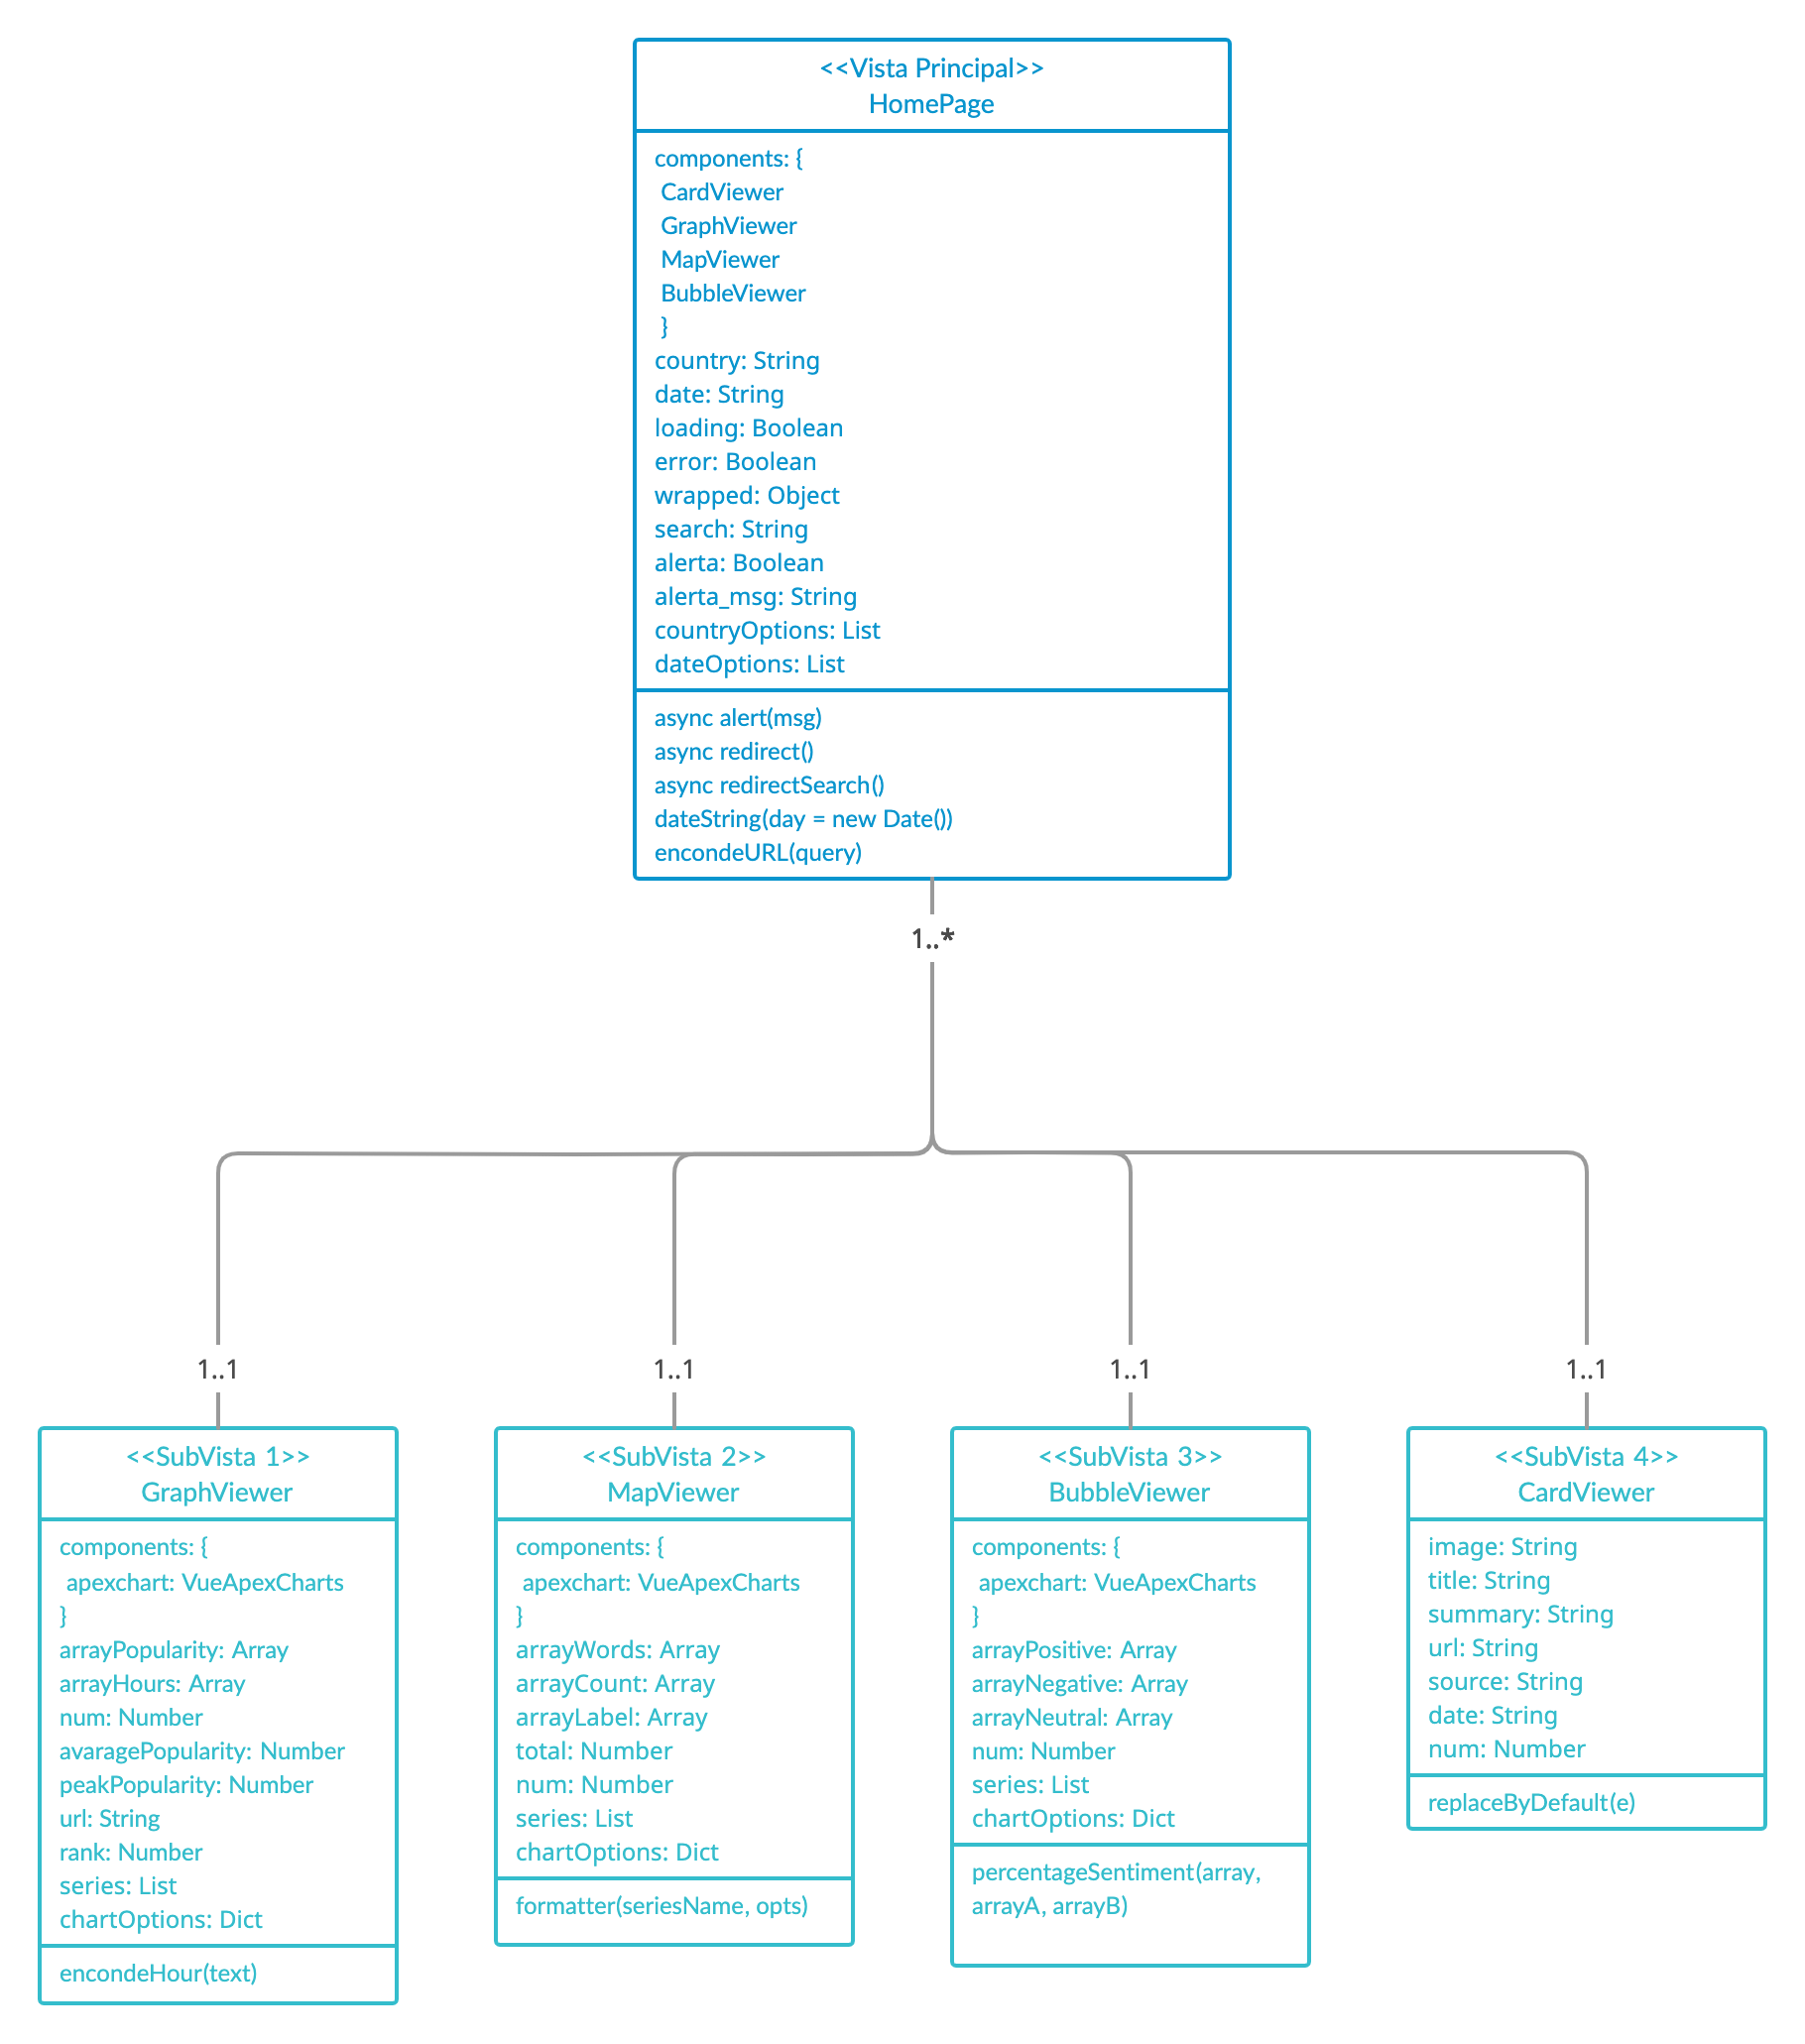
\includegraphics[width=1\textwidth]{gfx/Diagrama-de-Vistas.png}
    \caption[Diagrama de clase de las Vistas]{Diagrama de clase de las Vistas.}\label{gfx:Diagrama-de-Vistas}
\end{figure}

Cada subvista es llamada desde la vista principal, cada una con propiedades y funciones diferentes, ya que la representación de cada vista debe ser única y esencial.

\vspace{0.3cm}

La Vista principal representa la visualización de la historia de usuario que fue contemplada en el Sprint 2 (\ref{subs:sprint-2}) y esta relaciona con la entidad explicada en la sección \ref{subsub:ent-tendencia}. Esta vista es llamada \textit{HomePage} y está formada por \textit{components}, los cuales son las diferentes subvistas que se ha mencionado anteriormente. Los parámetros de las distintas rutas están referenciados por \textit{country}, \textit{date}, \textit{countryOptions} y \textit{dateOptions}, además las funciones de esta vista tienen el objetivo de construir los distintos formularios y los datos de la tendencia se cargarán en \textit{wrapped}.

\vspace{0.3cm}

También existen propiedades más complementarias como \textit{num} y \textit{rank}, para enumerar las tarjetas o cartas y el \textit{ranking} de la tendencia, respectivamente. Las funciones de alerta o los distintos atributos como \textit{loading}, existen para enriquecer las animaciones de la página y para mostrar el cuadro de dialogo que se ha mencionado anteriormente (\ref{gfx:boceto-error}). Finalmente, la función de \textit{encodeURL} codifica el nombre de la tendencia para redirigirlo a la plataforma Twitter mediante un enlace.

\subsection{Subvista Popularidad}
Esta subvista representa la visualización de las historias de usuario que fueron contempladas en el Sprint 6 (\ref{subs:sprint-6}). En ellas el usuario debe poder visualizar datos de interés sobre la popularidad y también un gráfica de área. La implementación de la gráfica se consigue mediante la librería ApexCharts.

\begin{figure}[H]
    \centering
    \myfloatalign
    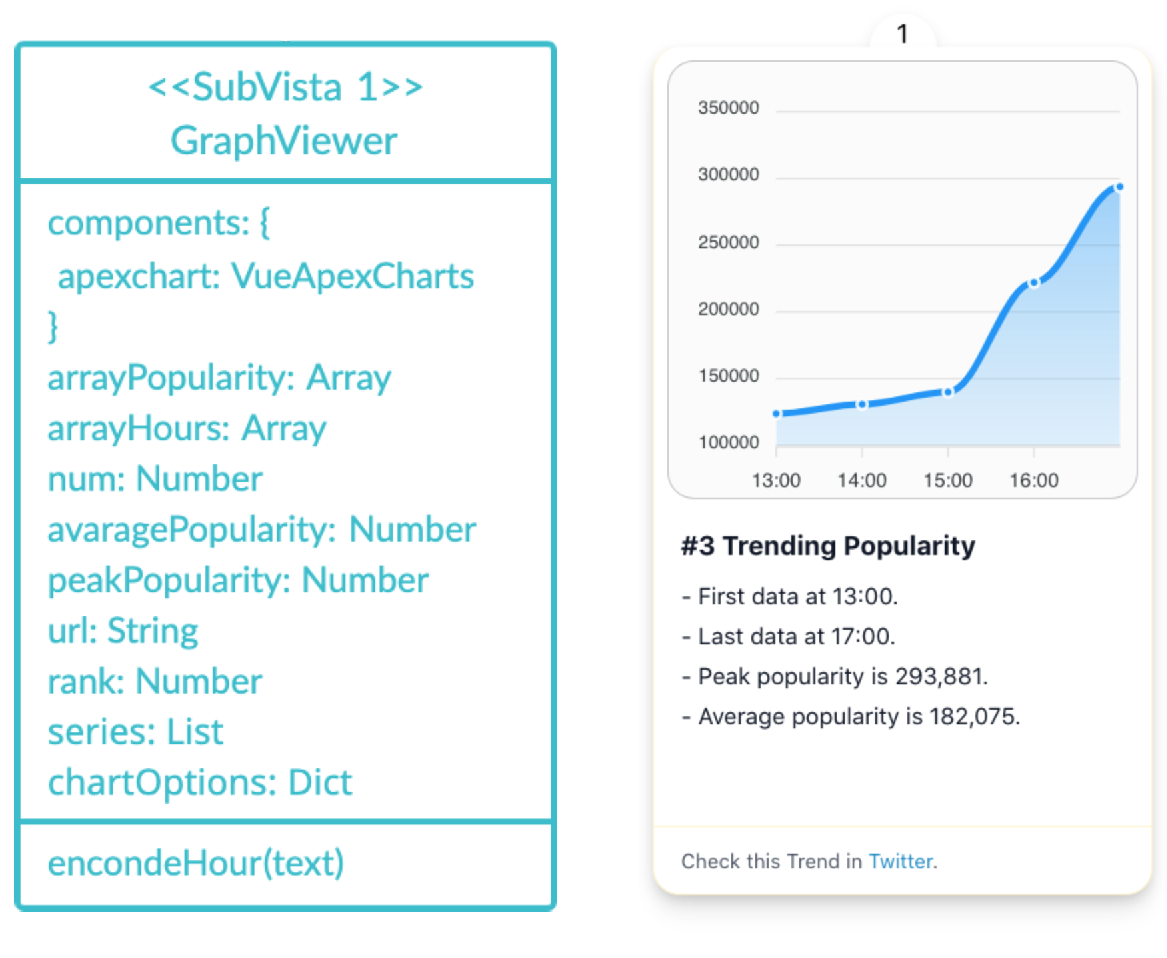
\includegraphics[width=0.9\textwidth]{gfx/subvista1.png}
    \caption[Estructura y Diseño de la primera subvista]{Estructura y Diseño de la primera subvista.}\label{gfx:subvista1}
\end{figure}

Los diferentes valores que posee esta subvista están relacionados con la entidad Popularidad (\ref{subsub:ent-popularidad}), a excepción de propiedades de la gráfica y atributos complementarios como \textit{url}, para redirigir a la plataforma de Twitter. La función debe transformar el texto en formato \textit{Date} de JavaScript.

\subsection{Subvista Palabras más Comunes y Keywords}
Esta subvista representa la visualización de las historias de usuario que fueron contempladas en el Sprint 7 (\ref{subs:sprint-7}). En ellas el usuario debe poder visualizar datos de interés sobre las palabras más comunes, las \textit{keywords} y un gráfico de radial de barras correspondiente. La implementación de la gráfica se consigue mediante la librería ApexCharts.

\begin{figure}[H]
    \centering
    \myfloatalign
    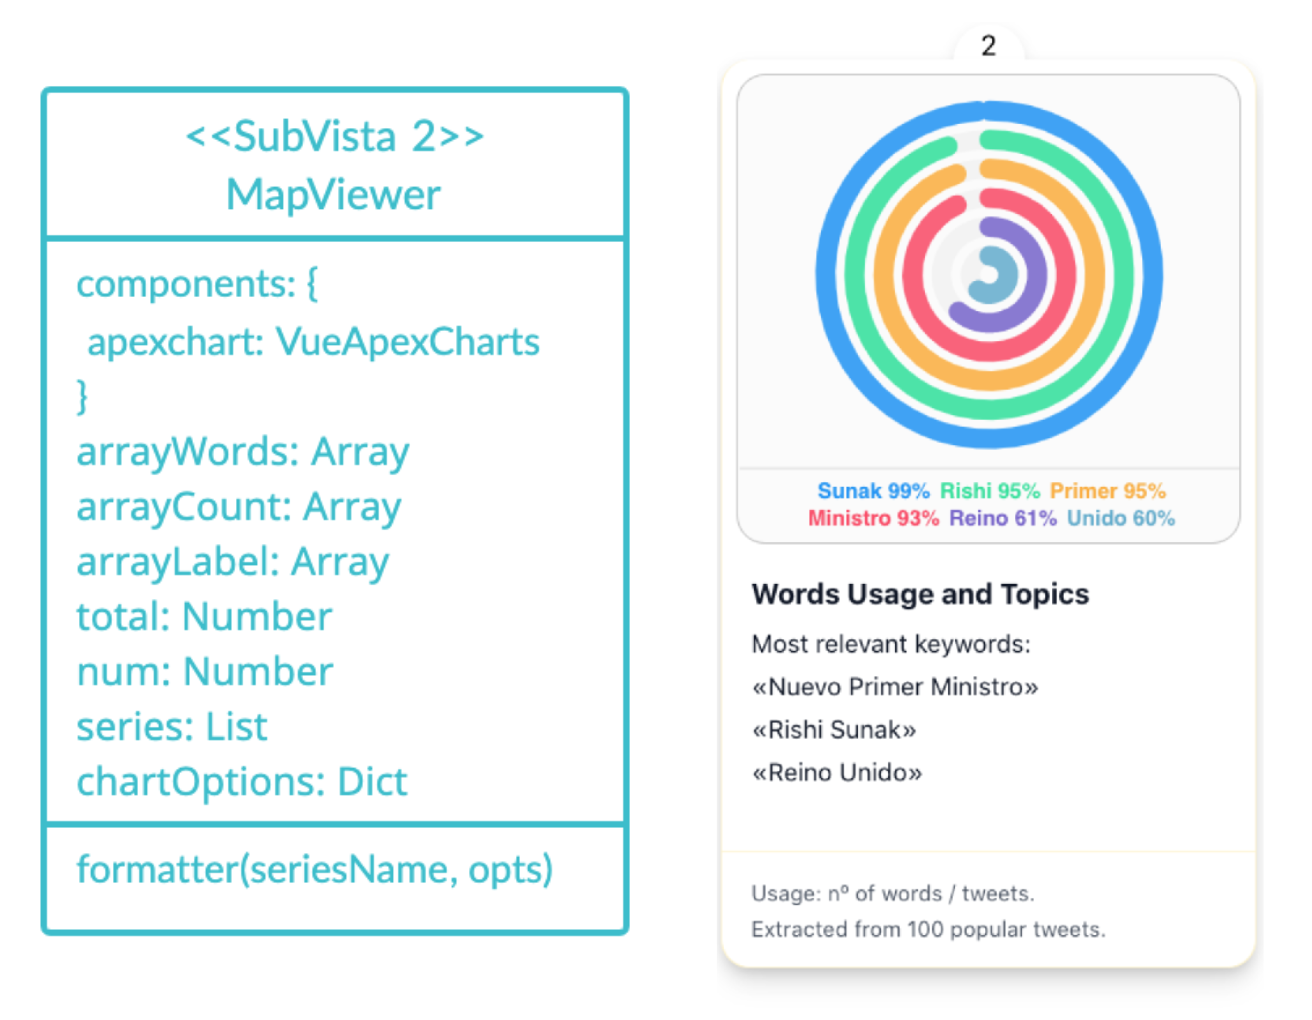
\includegraphics[width=0.9\textwidth]{gfx/subvista2.png}
    \caption[Estructura y Diseño de la segunda subvista]{Estructura y Diseño de la primera subvista.}\label{gfx:subvista2}
\end{figure}

Los diferentes valores que posee esta subvista están relacionados con la entidad explicada en la sección \ref{subsub:ent-keywords}. La función adapta el formato a los porcentajes.

\vspace{0.3cm}

Esta subvista tuvo un diseño inicial que fue descartado por problemas de diseño y también por posible confusión a la hora de interpretar el gráfico. El diseño tuvo problemas a la hora de encajar el gráfico en su encuadre y no quedaba muy claro el porcentaje de uso de las distintas palabras.

\begin{figure}[H]
    \centering
    \myfloatalign
    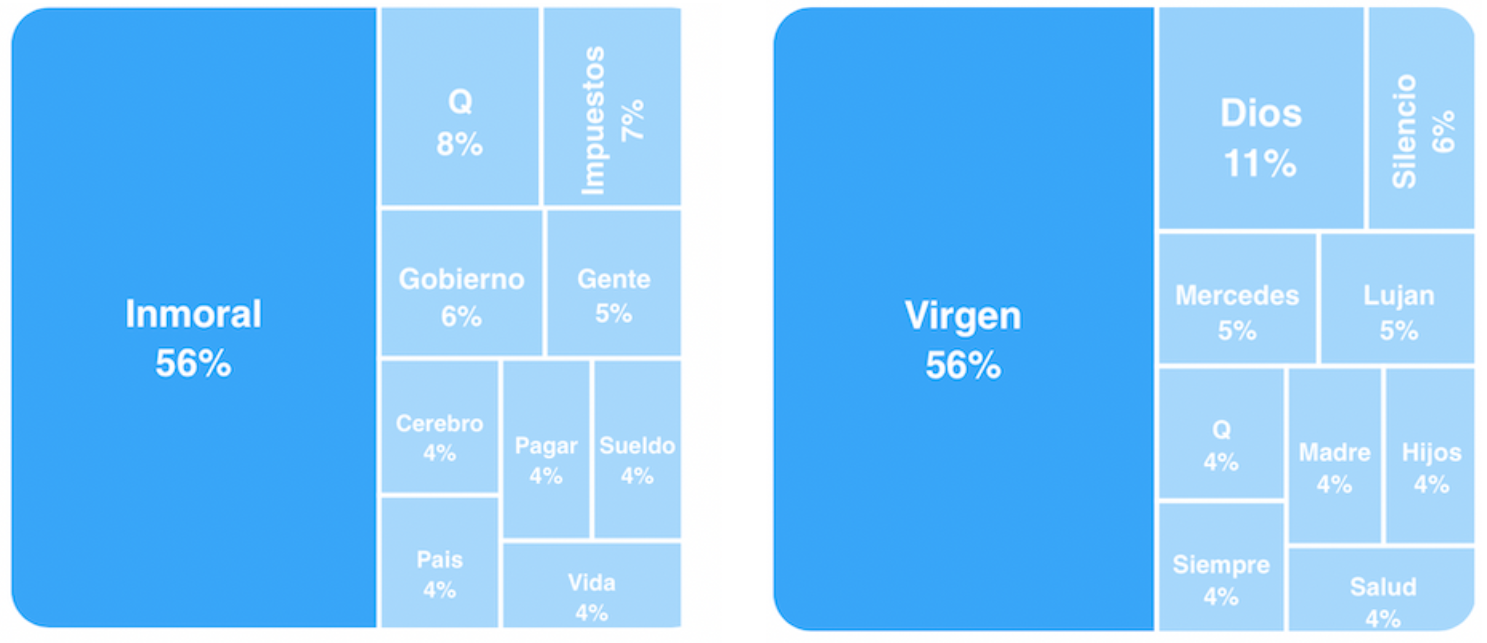
\includegraphics[width=0.8\textwidth]{gfx/subvista2-descartada.png}
    \caption[Diseño descartado de la segunda subvista]{Diseño descartado de la segunda subvista.}\label{gfx:subvista2-descartada}
\end{figure}

\subsection{Subvista Sentimiento General}
Esta subvista representa la visualización las historias de usuario que fueron contempladas en el Sprint 8 (\ref{subs:sprint-8}). En ellas el usuario debe poder visualizar datos de interés sobre el sentimiento general de los tweets o publicaciones y un gráfico de burbujas correspondiente. La implementación de la gráfica se consigue mediante la librería ApexCharts.

\begin{figure}[H]
    \centering
    \myfloatalign
    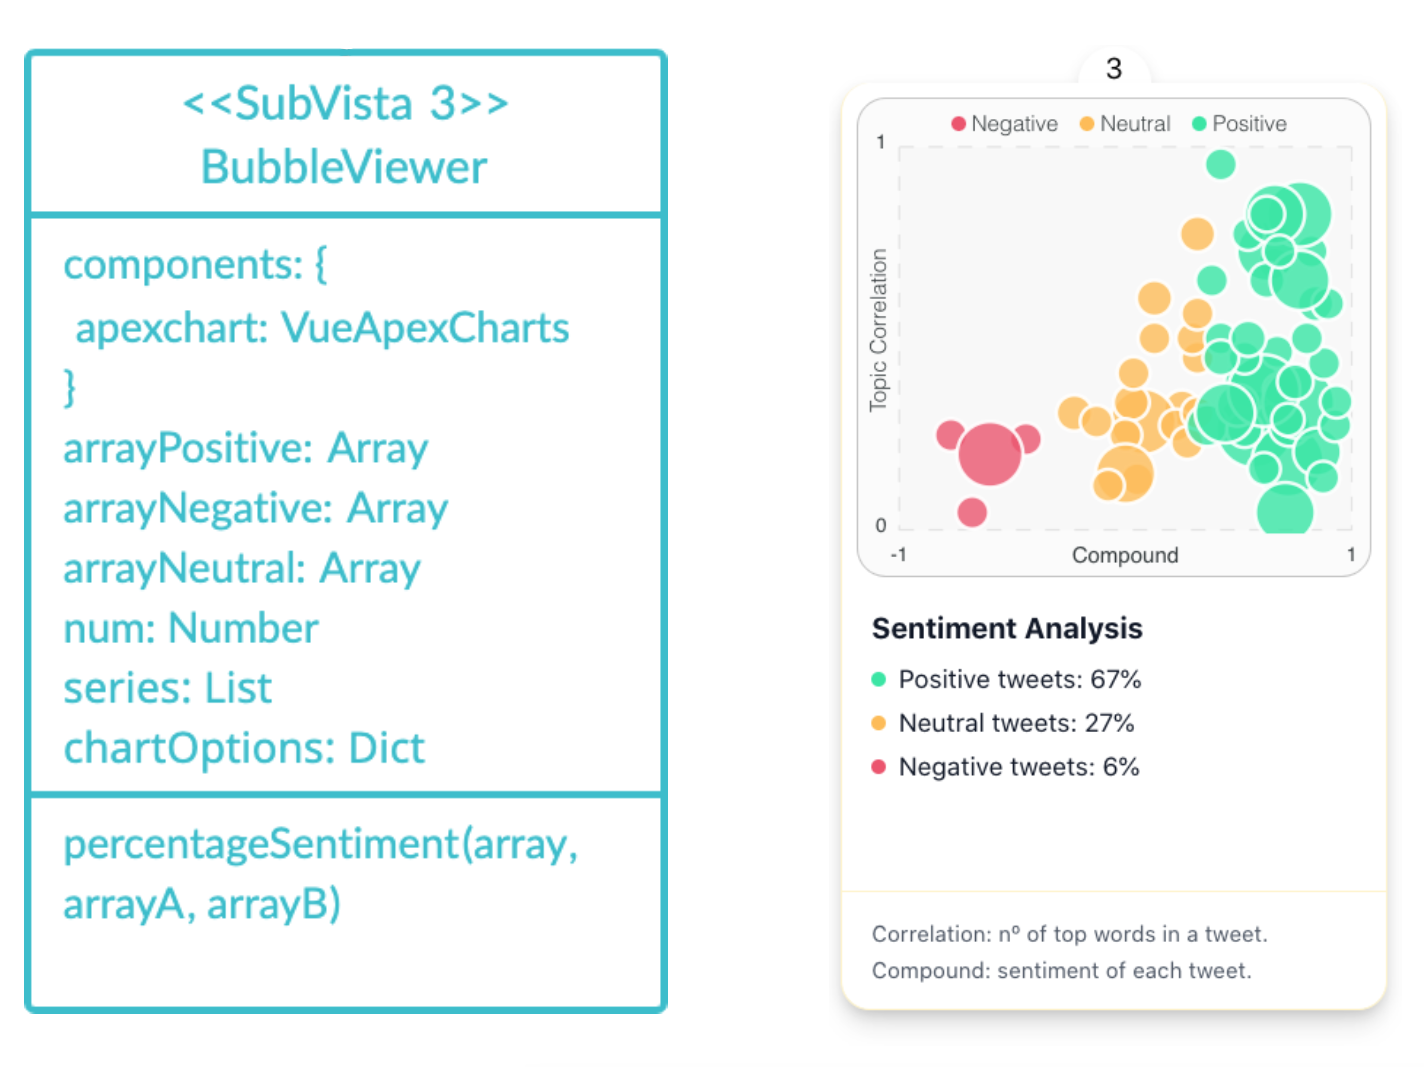
\includegraphics[width=0.9\textwidth]{gfx/subvista4.png}
    \caption[Estructura y Diseño de la tercera subvista]{Estructura y Diseño de la tercera subvista.}\label{gfx:subvista4}
\end{figure}

Los diferentes valores que posee esta subvista están relacionados con la entidad explicada en la sección \ref{subsub:ent-sentiment}. La función calcula el porcentaje dependiendo del radio de las burbujas.

\subsection{Subvista Noticas Relacionadas}
Esta subvista representa la visualización las historias de usuario que fueron contempladas en el Sprint 9 (\ref{subs:sprint-9}). En ellas el usuario debe poder visualizar datos de interés sobre las noticias o artículos relacionados sobre la tendencia.

\begin{figure}[H]
    \centering
    \myfloatalign
    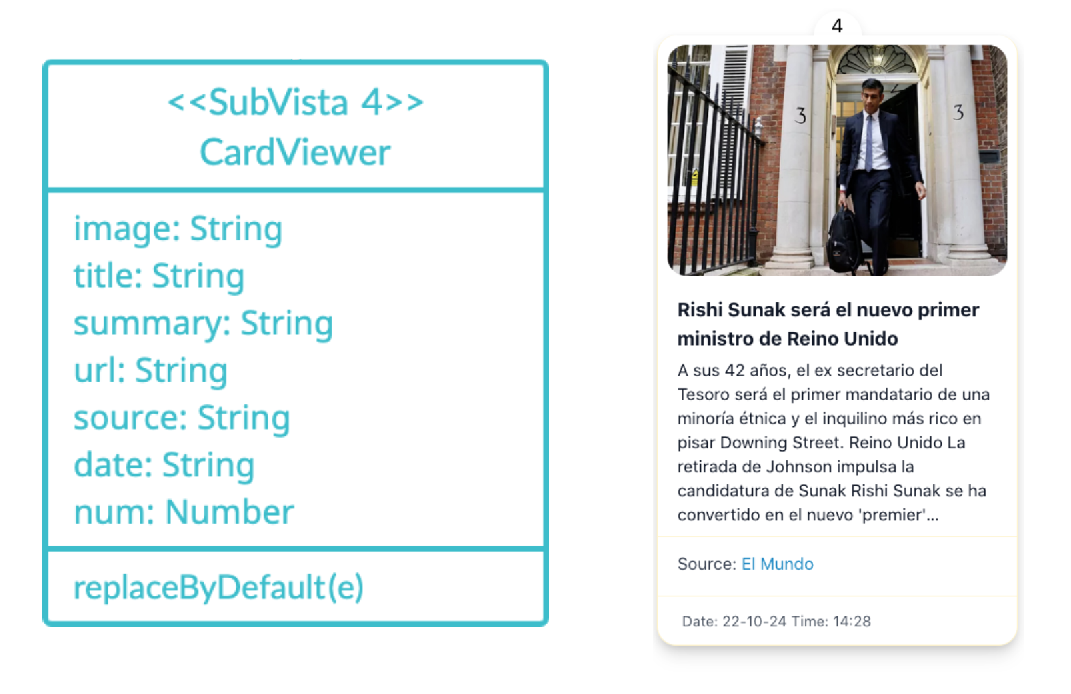
\includegraphics[width=0.9\textwidth]{gfx/subvista3.png}
    \caption[Estructura y Diseño de la última subvista]{Estructura y Diseño de la última subvista.}\label{gfx:subvista3}
\end{figure}

Los diferentes valores que posee esta subvista están relacionados con la entidad explicada en la sección \ref{subsub:ent-noticias}. La función devuelve una imagen por defecto si la carga de la imagen de la noticia falla.